\documentclass[oneside,12pt]{book}
\usepackage[utf8]{inputenc}
\usepackage{standalone}
\usepackage[margin=2.5cm]{geometry}
\usepackage{graphicx}
\usepackage{hyperref}
\usepackage{lmodern}
\usepackage{float}
\usepackage[spanish]{babel}
\usepackage{csquotes}
\usepackage[figurename=Ilustración]{caption}
\usepackage{enumitem}
\usepackage[numbers]{natbib}
\usepackage{ragged2e}
\usepackage{array}
\usepackage{multirow}
\usepackage{parskip}
\usepackage{listings}
\usepackage{epigraph}
\usepackage{booktabs}
\usepackage{longtable}

\usepackage{algorithm}
\usepackage{algpseudocode}

% Glosario de términos
\usepackage[acronym,nonumberlist]{glossaries}
\makeglossaries

% Viñetas cuadradas en todas las listas itemize
\usepackage{amssymb}
\renewcommand\labelitemi{$\blacksquare$}

% Otros paquetes y ajustes
\usepackage{geometry}
\usepackage{xcolor}

\renewcommand{\lstlistingname}{Algoritmo}
\floatname{algorithm}{Algoritmo}
\renewcommand{\listalgorithmname}{Índice de~\lstlistingname s}

\lstset{
        basicstyle=\fontsize{7}{11}\ttfamily,
        language=Java,
        captionpos=b,
}

\usepackage{titlesec}
\setcounter{secnumdepth}{3}
\titleformat{\chapter}[display]
{\normalfont\huge\bfseries}{\chaptertitlename\ \thechapter}{20pt}{\Huge}

\urlstyle{same}
\title{Sistema de Facturación: Aplicación Móvil Nativa para la Generación y Gestión de Facturas con Funcionalidades Avanzadas}
\author{Juan Carlos Acosta Perabá}
\date{Curso 20XX -- 20XX}
\renewcommand{\contentsname}{Contenido}
\renewcommand{\figurename}{Ilustración}

\begin{document}
%\maketitle
\begin{titlepage}

\begin{center}

\vspace*{0.25in}
\begin{figure}[htb]
\begin{center}

\includegraphics[width=15cm]{Ilustraciones/NuevoLogoEII.png}
%
\includegraphics[width=15cm]{Ilustraciones/LogoEII.jpg}
%
\includegraphics[width=20cm]{Ilustraciones/Logo_EII+ULPGC.png}
\end{center}
\end{figure}

\vspace*{0.25in}
\vspace*{0.25in}
\begin{Huge}
    \textbf{Trabajo de Fin de Grado} \\
\end{Huge}
\vspace*{0.5in}

\noindent\hfil\rule{17cm}{0.2mm}\hfil\\

\vspace*{0.1in}
\begin{Huge}
    \textbf{Sistema de Facturación: Aplicación Móvil Nativa para la Generación y Gestión de Facturas con Funcionalidades Avanzadas} \\
\end{Huge}
\vspace*{0.3in}
\begin{large}
TITULACIÓN: \\
Grado en Ingeniería Informática \\
\vspace*{0.1in}
AUTOR: \\
Juan Carlos Acosta Perabá \\
\end{large}
\vspace*{0.3in}
\noindent\hfil\rule{17cm}{0.2mm}\hfil\\
\vspace*{0.1in}
\begin{large}
TUTORIZADO POR: \\
María Dolores Afonso Suárez \\
\end{large}
\vspace*{0.3in}
Junio de 2025

\end{center}


\end{titlepage}


\newgeometry{margin=1.5cm}

\thispagestyle{empty}

%\lhead{ 
\begin{tabular}{p{15cm}p{5cm}}
  %
\includegraphics{Ilustraciones/LogoEII.jpg}   &  TFT04\\
  
\includegraphics[width=7cm]{Ilustraciones/NuevoLogoEII.png}   &  TFT04\\
\end{tabular}
%}

\vspace{1em}
\fboxrule=2pt
\begin{center}
\fcolorbox{gray}{gray!10}{\parbox{.8 \textwidth}{ {\large SOLICITUD DE DEFENSA DE TRABAJO DE FIN DE TÍTULO}}}
\end{center}

\vspace{1em}
\justify
D./Dª Juan Carlos Acosta Perabá, autor del trabajo Sistema de Facturación: Aplicación Móvil Nativa para la Generación y Gestión de Facturas con Funcionalidades Avanzadas, correspondiente a la titulación Grado en Ingeniería Informática

\vspace{1em}
SOLICITA

\vspace{1em}
que se inicie el procedimiento de defensa del mismo, para lo que se adjunta la documentación requerida, haciendo constar que 

[x] se autoriza / [ ] no se autoriza la grabación en audio de la exposición y turno de preguntas.

\vspace{1em}
Asimismo, con respecto al registro de la propiedad intelectual/industrial del TFT, declara que:

[ ] Se ha iniciado o hay intención de iniciarlo (defensa no pública).

[x] No está previsto.

\vspace{1em}
Y para que así conste firma la presente. (fecha en firma electrónica)

\begin{center}
%En Las Palmas de Gran Canaria, a día de mes de año

\vspace{1em}
El/La estudiante

\vspace{3em}
Fdo.------------------------
\end{center}

\begin{center}
\fcolorbox{gray}{white!10}{\parbox{.9\textwidth}{
{\tiny A rellenar y firmar \textbf{obligatoriamente} por el/la/los/las tutores}

En relación con la presente solicitud, se informa:{\tiny (firmar donde corresponda)}

\vspace{1em}
\begin{center}
\begin{tabular}{|p{\dimexpr.45\linewidth}|p{\dimexpr.45\linewidth}|}
%\begin{tabular}{|l|r|}
    \hline
   & \\
  Positivamente {\tiny (en  caso  de  detección  de  copia, esta firma quedará invalidada)}  & Negativamente {\tiny (justificación en TFT05)} \\
   & \\
   & \\
   & \\
   & \\
   & \\
   & \\
  Fdo.------------------------ & Fdo.------------------------  \\
     & \\

    \hline
\end{tabular} 

\end{center}

\vspace{1em}

}
}

\vspace{1em}

%\cfoot{
DIRECTOR DE LA ESCUELA DE INGENIERÍA INFORMÁTICA
%}

\end{center}

\restoregeometry

\clearpage

\newpage
\pagenumbering{roman}
{\Large{\textbf{Agradecimientos}}}
\begin{flushright}
\Large\itshape
En primer lugar, deseo expresar mi más profundo agradecimiento a mis padres, a mi hermana, a mi pareja y a mis amigos por su apoyo incondicional a lo largo de este arduo camino, por acompañarme y levantarme cada vez que sentí que no podía más.

Agradezco asimismo a la persona que me guió en este proyecto por su paciencia inquebrantable y la confianza que depositó en mí.

Finalmente, gracias a todas las personas que, de una u otra forma, hicieron posible que llegara hasta aquí.

Muchas gracias.
\end{flushright}

\clearpage
% Ajuste global (si aún no lo tenías)
\setlength{\parskip}{8mm}

% -------------- Resumen --------------
\section*{Resumen}

{\large
Este Trabajo de Fin de Grado presenta una aplicación móvil nativa, complementada por un portal web, para la gestión integral de la facturación de empresas y autónomos. La plataforma centraliza facturas, empleados y clientes; permite registrar negocios, crear cuentas para el personal y ofrecer a los clientes acceso directo a sus documentos. Incluye generación de facturas mediante formularios dinámicos, almacenamiento en la nube, exportación PDF, trabajo offline con sincronización posterior y notificaciones automáticas. La herramienta mejora la eficiencia y accesibilidad del proceso, reduce la dependencia del papel y aporta una solución moderna, segura y alineada con las necesidades actuales de la gestión empresarial.
}

\newpage

% -------------- Abstract --------------
\section*{Abstract}

{\large
This Final Degree Project presents a native mobile application, complemented by a web portal, for comprehensive invoicing management for businesses and freelancers. The platform centralises invoices, employees and clients; it lets owners register their company, create staff accounts and grant customers direct access to their documents. Features include invoice generation through dynamic forms, cloud storage, PDF export, offline work with later synchronisation and automatic notifications. The tool enhances efficiency and accessibility in invoicing, reduces reliance on paper and provides a modern, secure solution aligned with current business management needs.
}
\tableofcontents

\renewcommand{\lstlistlistingname}{Bloques de código}
\lstlistoflistings
\listoffigures
\listoftables

\clearpage
\pagenumbering{arabic}

% 1. Introducción
\chapter{Introducción}
%----------------------------------------------------------
% Capítulo 1 – Introducción
%----------------------------------------------------------
\epigraph{Si enciendes una lámpara para alguien, iluminas también tu propio camino.}{Buda}

\begin{large}
  
La facturación es uno de los cimientos de la actividad económica: registra las operaciones comerciales, permite el control fiscal y protege los derechos de compradores y vendedores. A lo largo de la historia, desde las tablillas mesopotámicas hasta las facturas digitales que circulan hoy día, la tecnología ha perfeccionado este proceso para garantizar disponibilidad, autenticidad e integridad de la información \cite{origen_facturas}.

En España, la \textbf{Ley 18/2022 de Creación y Crecimiento Empresarial} ha acelerado esta transición al imponer la factura electrónica en todas las operaciones \gls{b2b}. Las grandes empresas ya la aplican de forma obligatoria y, para pymes y autónomos, la exigencia será plena a lo largo de 2025 \cite{ley18_2022}. Al mismo tiempo, la expansión del trabajo remoto y el uso extendido de dispositivos móviles han mostrado claramente la diferencia que existe entre los programas de escritorio tradicionales y las necesidades actuales de movilidad.

En este trabajo se aborda ese desafío mediante un sistema de facturación centrado en aplicaciones móviles nativas (iOS y Android) junto con un panel administrativo web.

\end{large}

%----------------------------------------------------------
\section{Motivación y antecedentes}
%----------------------------------------------------------

\begin{large}

La gestión de facturas en la pequeña y mediana empresa sigue apoyándose, en gran medida, en un conjunto de soluciones aisladas: sistemas \gls{erp} de sobremesa, hojas de cálculo improvisadas y repositorios documentales que raramente se comunican entre sí. Esta fragmentación causa que los datos se dupliquen y dificulta la colaboración directa entre empresario, personal interno y cliente final.

Al mismo tiempo, el auge de los servicios \gls{saas} ha desplazado el trabajo contable a la nube; sin embargo, muchos de estos portales exigen conectividad permanente para funcionar. En zonas con cobertura deficiente, la emisión o actualización de facturas se retrasa, lo que genera cuellos de botella y pone en riesgo la puntualidad de la información.

La obligatoriedad próxima de la factura electrónica, recogida en la Ley 18/2022, obliga a las pymes y autónomos a actualizar sus procesos administrativos para adaptarse plenamente antes de 2025.

Por último, la movilidad se ha consolidado como requisito operativo. Según el \enquote{2023 Mid‐market Technology Trends Report} de Deloitte, la mayoría de las empresas de tamaño medio ofrece hoy acceso a sus plataformas de gestión desde dispositivos móviles, aunque con frecuencia esas aplicaciones replican solo las funciones básicas de escritorio \cite{estudio_movilidad}.

\end{large}

%----------------------------------------------------------
\section{Objetivos}
%----------------------------------------------------------

\subsection{Objetivo general}

\begin{large}

El objetivo general es desarrollar una plataforma integral de facturación con aplicaciones móviles nativas para iOS y Android, complementadas por un portal web administrativo. La solución debe operar sin interrupciones, incluso en ausencia de conexión, y ofrecer una experiencia de uso clara, accesible y satisfactoria.

\end{large}

%----------------------------------------------------------
\subsection{Objetivos específicos}
%----------------------------------------------------------

\begin{large}

Los objetivos específicos que guían el desarrollo del proyecto son:

En primer lugar se plantea el diseño de una arquitectura de datos sólida que represente con precisión las entidades del dominio, es decir, empresas, usuarios y facturas, y permita la evolución y el mantenimiento del sistema sin inconsistencias.

El segundo objetivo establece la implantación de un mecanismo de autenticación y autorización que gestione roles y permisos con rigor, de manera que cada perfil acceda únicamente a las funciones que le correspondan.

El tercer objetivo se centra en desarrollar la lógica de generación automática de facturas, incorporando el cálculo exacto de impuestos y la exportación de los documentos a PDF con calidad profesional y compatibilidad con los estándares de facturación electrónica.

El cuarto objetivo persigue proporcionar a la plataforma un modo de funcionamiento sin conexión que posibilite crear o modificar facturas en entornos offline y sincronizar los cambios en cuanto se restablezca la conectividad.

El quinto objetivo aborda la construcción de un portal web administrativo con cuadros de mando y métricas financieras detalladas, cuyo propósito es facilitar el seguimiento de ingresos, gastos y morosidad y respaldar la toma de decisiones.

Por último, el sexto objetivo apunta a proteger la confidencialidad e integridad de la información mediante cifrado tanto en tránsito como en reposo, garantizando el cumplimiento de los requisitos establecidos por el \gls{rgpd}.

\end{large}

%----------------------------------------------------------
\section{Competencias específicas}
%----------------------------------------------------------

\begin{large}

El desarrollo de este proyecto ha requerido poner en práctica un conjunto de competencias técnicas directamente relacionadas con el diseño, implementación y evaluación de sistemas de información avanzados. A continuación se detallan las competencias específicas que se han puesto en práctica a lo largo de la realización de este trabajo:

\begin{itemize}[label=\raisebox{0.15ex}{\scriptsize$\blacksquare$}]
  \item \textbf{CI1.} Capacidad para diseñar, desarrollar, seleccionar y evaluar aplicaciones y sistemas informáticos, asegurando su fiabilidad y calidad.
  \item \textbf{CI2.} Aptitud para planificar, concebir y dirigir proyectos y servicios informáticos a lo largo de todo su ciclo de vida.
  \item \textbf{CI3.} Conocimiento de las métricas de calidad y los procesos de mejora continua aplicados al software.
  \item \textbf{CI5.} Capacidad para comprender, aplicar y mantener los principios de ingeniería de requisitos.
  \item \textbf{CI6.} Habilidad para diseñar y gestionar bases de datos y servicios en la nube, garantizando integridad y disponibilidad de la información.
  \item \textbf{CI8.} Competencia para analizar, construir y mantener aplicaciones robustas y eficientes, eligiendo los lenguajes y paradigmas más adecuados.
  \item \textbf{CI12.} Conocimiento y aplicación de las estructuras de datos y su impacto en el rendimiento del sistema.
  \item \textbf{CI16.} Aplicación de los principios y metodologías de la ingeniería del software para asegurar procesos ordenados de desarrollo y mantenimiento.
  \item \textbf{CI17.} Capacidad para diseñar y evaluar interfaces persona–computador que garanticen accesibilidad y usabilidad.
  \item \textbf{TI1.} Comprensión del entorno de una organización y de sus necesidades en materia de tecnologías de la información.
  \item \textbf{TI2.} Capacidad para seleccionar, desplegar e integrar tecnologías de hardware, software y redes dentro de los parámetros de calidad adecuados.
  \item \textbf{TI3.} Uso de metodologías centradas en el usuario y la organización para el desarrollo y la evaluación de aplicaciones.
  \item \textbf{TI5.} Capacidad para seleccionar, integrar y gestionar sistemas de información que satisfagan los requisitos de la organización.
  \item \textbf{TI6.} Capacidad para concebir sistemas, aplicaciones y servicios basados en tecnologías de red, incluidos entornos web y móviles.
  \item \textbf{TI7.} Aptitud para aplicar y gestionar la garantía y la seguridad de los sistemas de información.
\end{itemize}

Estos conocimientos y habilidades, extraídos directamente del plan de estudios oficial, han sido fundamentales para llevar a cabo el análisis, diseño e implementación de la plataforma de facturación propuesta \cite{grado2024ulpgc}.

\end{large}

%----------------------------------------------------------
\section{Alineamiento con los Objetivos de Desarrollo Sostenible}
%----------------------------------------------------------

\begin{large}

\begin{table}[H]
\caption{Grado de relación del TFT con los objetivos de desarrollo sostenible.}
\label{tab:ODS}
\centering
\begin{tabular}{|l|c|c|c|c|}
\cline{1-5}
 & \multicolumn{4}{c|}{Grado de relación} \\ \cline{2-5}
ODS & 0 No procede & 1 Bajo & 2 Medio & 3 Alto \\ \cline{1-5}
1 Fin de la Pobreza                & X &   &   &   \\ \cline{1-5}
2 Hambre cero                      & X &   &   &   \\ \cline{1-5}
3 Salud y Bienestar                & X &   &   &   \\ \cline{1-5}
4 Educación de calidad             & X &   &   &   \\ \cline{1-5}
5 Igualdad de género               & X &   &   &   \\ \cline{1-5}
6 Agua limpia y saneamiento        & X &   &   &   \\ \cline{1-5}
7 Energía asequible y no contaminante & X &   &   &   \\ \cline{1-5}
8 Trabajo decente y crecimiento económico & X &   &   &   \\ \cline{1-5}
9 Industria, innovación e infraestructuras &   &   &   & X \\ \cline{1-5}
10 Reducción de las desigualdades  &   & X &   &   \\ \cline{1-5}
11 Ciudades y comunidades sostenibles &   &   & X &   \\ \cline{1-5}
12 Producción y consumo responsables &   &   & X &   \\ \cline{1-5} 
13 Acción por el clima             &   & X &   &   \\ \cline{1-5}
14 Vida submarina                  & X &   &   &   \\ \cline{1-5}
15 Vida de ecosistemas terrestres  & X &   &   &   \\ \cline{1-5}
16 Paz, justicia e instituciones sólidas & X &   &   &   \\ \cline{1-5}
17 Alianzas para lograr objetivos  & X &   &   &   \\ \cline{1-5}
\end{tabular}
\end{table}

En primer lugar, en relación con el \textbf{ODS 9 – Industria, innovación e infraestructuras}, la aplicación propone una infraestructura digital accesible, capaz de operar sin conexión para garantizar la continuidad del negocio en entornos con conectividad limitada. Además, sus funciones de generación y exportación de facturas en PDF modernizan los procesos administrativos. 

Respecto al \textbf{ODS 10 – Reducción de las desigualdades}, el diseño centrado en la usabilidad del teléfono móvil facilita que microempresas y autónomos, con recursos más reducidos, puedan adoptar tecnología avanzada de facturación, reduciendo la brecha digital frente a grandes organizaciones. 

En cuanto al \textbf{ODS 11 – Ciudades y comunidades sostenibles}, la eliminación del papel y la eliminación de desplazamientos para la entrega física de documentos contribuye a disminuir residuos urbanos y a apoyar la sostenibilidad económica y medioambiental de los comercios locales. 

El \textbf{ODS 12 – Producción y consumo responsables} se ve favorecido al sustituir procesos basados en facturas impresas por archivos cifrados en la nube, promoviendo prácticas \textit{paper-less} y un uso más eficiente de los recursos materiales y energéticos. 

Finalmente, el \textbf{ODS 13 – Acción por el clima} recibe un impulso gracias a la reducción del consumo de papel y de envíos postales, lo que disminuye la huella de carbono administrativa. Aunque el uso de dispositivos móviles y servicios en la nube conlleva consumo energético, el balance de emisiones es muy inferior al de los métodos tradicionales, siempre que se adopten buenas prácticas de eficiencia energética.

\end{large}

% 2. Análisis
\chapter{Análisis}
%----------------------------------------------------------
% Capítulo 2 – Análisis
%----------------------------------------------------------

%----------------------------------------------------------
\section{Problema}
%----------------------------------------------------------

\begin{large}

El día a día de muchas pymes y autónomos sigue un recorrido fragmentado, combinando plantillas en hojas de cálculo, correos electrónicos y archivado físico. Esta fragmentación obliga a reintroducir datos manualmente en varias aplicaciones, aumentando el riesgo de errores humanos e inconsistencias, dificultando la obtención de información financiera fiable y generando retrasos en los cobros y pagos. Además, la falta de conectividad estable limita gravemente la movilidad, impidiendo emitir o consultar facturas en tiempo real, provocando que la información quede rápidamente obsoleta.

A esto se suman las exigencias normativas recientes, como la Ley 18/2022, que obliga a las empresas a emitir factura electrónica en todas sus transacciones comerciales, mantener registros íntegros y garantizar la autenticidad de cada documento. Cumplir con estos requisitos con herramientas tradicionales implica una inversión considerable en nuevas soluciones, formación del personal y rediseño de procesos internos, afectando negativamente la productividad, la competitividad y el potencial de crecimiento de los negocios.

\end{large}

%----------------------------------------------------------
\section{Solución}
%----------------------------------------------------------

\begin{large}

Se propone una plataforma de facturación basada en aplicaciones móviles nativas para iOS y Android y un portal web administrativo. Todas las versiones se conectan a Firestore, lo que garantiza la consistencia de los datos. Firebase actúa como backend sin servidor, reduciendo la carga de mantenimiento y permitiendo un escalado automático según el uso.

Las apps móviles siguen un modelo \textit{offline-first}: cuando no hay conexión, los datos se almacenan localmente de forma segura y se sincronizan con Firestore tan pronto se restablece la red. Así, se puede seguir trabajando sin interrupciones y los posibles conflictos se resuelven automáticamente mediante marcas de tiempo.

Se plantea utilizar Cloud Functions para generar los PDF de las facturas, aplicar numeración secuencial y almacenar los archivos en Cloud Storage. La seguridad está cubiera con reglas de Firestore, autenticación y cifrado, cumpliendo con el \gls{rgpd} y dejando registro de auditoría para cada operación sensible.

El portal web, construido con \gls{astro} y alojado en Vercel, muestra en tiempo real indicadores clave (ingresos cobrados, importes pendientes, ratio de morosidad). Gracias a la suscripción en tiempo real a Firestore y al enfoque de generar HTML estático en el servidor y habilitar la hidratación únicamente en los componentes que lo requieren, la interfaz permanece ligera, accesible y adaptable a distintos dispositivos. En conjunto, esta solución unifica el flujo de trabajo, elimina la fragmentación de herramientas y permite facturar desde cualquier lugar, reduciendo costes operativos y minimizando errores.

\end{large}

%----------------------------------------------------------
\section{Metodología}
%----------------------------------------------------------

\begin{large}

Para desarrollar la plataforma se adoptó un enfoque ágil iterativo incremental basado en Kanban. Cada tarea se crea y prioriza en GitHub Projects, limitando el trabajo en curso para enfocarnos en entregas parciales y ajustando el alcance según sea necesario.

El plan de trabajo se estructuró en siete fases bien diferenciadas: una \textbf{planificación inicial}; cinco \textbf{incrementos funcionales}; y una fase final de \textbf{documentación y presentación}. Cada incremento funcional se subdividió de forma repetible en las cuatro tareas que se describen a continuación:

\begin{itemize}
  \item \textbf{Análisis:} Detallamos funcionalidades y criterios de aceptación para cada incremento.
  \item \textbf{Diseño:} Definimos la arquitectura de datos y creamos prototipos de interfaz en Figma.
  \item \textbf{Implementación:} Desarrollamos la app para iOS y Android, escribimos las funciones de backend y construimos el portal web.  
  \item \textbf{Pruebas:} Realizamos pruebas manuales en dispositivos emulados para verificar que cada función cumple los requisitos.
\end{itemize}

Al finalizar los cinco incrementos funcionales se dedicó tiempo a la elaboración de la documentación completa: manuales de usuario, guía de despliegue y la memoria técnica. Durante esta etapa se generaron capturas y métricas que respaldan los resultados.

Con este esquema iterativo avanzamos de forma progresiva, mantuvimos la calidad en cada entrega y pudimos incorporar mejoras o ajustes cuando surgían nuevos requisitos.

\end{large}

%----------------------------------------------------------
\section{Marco de trabajo}
%----------------------------------------------------------

\begin{large}

El marco de trabajo del proyecto se articula en dos grandes componentes: los clientes nativos y el portal web. Cada uno cumple una función específica dentro del flujo integral de facturación:

\end{large}

\subsection{App iOS (\textit{Swift})}

\begin{large}

El código de la aplicación iOS sigue el patrón Model–View–ViewModel (MVVM) para separar lógicamente la interfaz de usuario de la capa de datos y negocio. 
\begin{itemize}
  \item \textbf{Modelo (Model):} Contiene las estructuras que representan entidades como Empresas, Clientes y Facturas. Estas estructuras definen los campos que se almacenan en Firestore (por ejemplo, fecha de emisión, importe, estado, etc.) y métodos para convertir documentos de Firestore a objetos Swift.
  \item \textbf{Vista (View):} Con SwiftUI se crearon vistas reutilizables para cada pantalla principal: lista de facturas, detalle de factura, formulario de creación/edición y ajustes. Cada vista se conecta a su ViewModel mediante propiedades marcadas con \textit{@ObservedObject} o \textit{@StateObject}.
  \item \textbf{ViewModel:} Cada pantalla tiene un ViewModel que agrupa la lógica de negocio y la interacción con Firebase. Los ViewModels se encargan de:
    \begin{itemize}
      \item Recuperar y observar los cambios en documentos de Firestore.
      \item Validar y formatear datos antes de mostrarlos en pantalla.
      \item Enviar nuevas facturas a Firestore, gestionar el estado (Paid/Pending) y calcular totales.
      \item Generar el PDF de la factura y guardarlo localmente, empleando el ID único de Firestore para numeración.
    \end{itemize}
  \item \textbf{Servicios de Firebase:}  
    \begin{itemize}
      \item \textit{Firestore:} Actúa como base de datos de documentos. Cada colección almacena objetos con la información necesaria.
      \item \textit{Authentication:} Gestiona el inicio de sesión con correo/contraseña, manteniendo sesiones y seguridad.
    \end{itemize}
\end{itemize}

\end{large}

\subsection{App Android (Kotlin)}

\begin{large}

La versión para Android estaba prevista en Kotlin siguiendo una arquitectura similar (MVVM), pero debido a limitaciones de tiempo no llegó a completarse. La carpeta \textit{android/} contiene el esqueleto del proyecto (configuración de Gradle, dependencias de Firebase, diseño de pantallas básicas), pero las funciones principales (CRUD de facturas, generación de PDF, lógica de sincronización) quedaron pendientes y se documentan como trabajo futuro.

\end{large}

\subsection{Portal Web (Astro)}

\begin{large}

El portal web se desarrolló con el framework Astro y estilos en TailwindCSS. La estructura principal del código es:
\begin{itemize}
  \item \textbf{Páginas estáticas (`/src/pages`):}  
    \begin{itemize}
      \item \textit{index.astro}: Página de inicio que contiene la gráfica donde se muestra el total de los pagado y de lo que queda pendiente de pago mensualmente.
      \item \textit{login.astro}: Página para que los usuarios, previamente registrados desde la aplicación móvil, puedan acceder con sus credenciales.
    \end{itemize}
  \item \textbf{Componentes (`/src/components`):}  
    \begin{itemize}
      \item \textit{ButtonToScrollToTop.astro}: Componente que renderiza un botón en la esquina inferior derecha de la página para volver al inicio de la página.
      \item \textit{Header.astro}: Componente que renderiza la cabecera de la página con un enlace de la web, un menú de navegación entre las diferentes secciones y el botón de cerrar la sesión.
      \item \textit{MoneyChart.astro}: Componente que renderiza la gráfica de barras usando \textit{lightweight-charts}.
      \item \textit{OverdueList.astro}: Componente que renderiza el listado de los clientes que no han pagado en su tiempo (morosos), haciendo el cálculo de la cantidad total que deben.
    \end{itemize}
  \item \textbf{Servicios de Firebase (en `/src/firebase`):}  
    \begin{itemize}
      \item \textit{config.ts}: Fichero con la configuración para establecer la conexión con firebase.
      \item \textit{firebase.ts}: Inicializa la instancia de Firebase y exporta funciones para autenticar y leer cualquier dato de Firestore.
    \end{itemize}
  \item \textbf{Despliegue:}  
    \begin{itemize}
      \item El portal web se publica en Vercel, con integración continua vía GitHub Actions. Cada merge a `main` dispara un despliegue automático.
    \end{itemize}
\end{itemize}

\end{large}

%----------------------------------------------------------
\section{Herramientas}
%----------------------------------------------------------

\begin{large}

En este proyecto hemos elegido herramientas que permitan un flujo de trabajo ágil y tecnológico acorde al alcance de la plataforma:

\end{large}

\subsection{iOS}

\begin{large}

Para la app de iPhone se utiliza \textbf{Swift}, un lenguaje moderno que destaca por su seguridad (tipado fuerte y gestión automática de memoria) y buen rendimiento gracias a sus compiladores optimizados \cite{swift_lang2025}. El desarrollo se lleva a cabo en \textbf{Xcode} 16.3, que combina editor, depurador y simulador de dispositivos. Además, Instruments facilita perfilar CPU, memoria y consumo energético, lo que ayuda a mejorar la fluidez de la interfaz. Con SwiftUI, se construyen vistas reutilizables que interactúan con los ViewModels, separando claramente la lógica de negocio de la presentación.

\end{large}

\subsection{Android}

\begin{large}

La versión para Android se prediseñó en \textbf{Kotlin} con una arquitectura MVVM similar a la de iOS, aprovechando su sintaxis concisa, el manejo seguro de nulabilidad y las corrutinas para tareas asíncronas \cite{kotlin_lang2025}. El entorno de trabajo es \textbf{Android Studio} 2024.3.2 (Meerkat Feature Drop), que incluye emuladores configurables, herramientas para inspeccionar bases de datos y analizadores de rendimiento en tiempo real \cite{as2024_3_2}. En esta primera iteración el esqueleto del proyecto está preparado, aunque las funcionalidades principales se documentan para futuras versiones.

\end{large}

\subsection{Web}

\begin{large}

El portal administrativo se desarrolla con \textbf{Astro}, que genera HTML estático en tiempo de compilación y aplica hidratación sólo donde se necesita, lo que reduce el tamaño inicial y mejora el rendimiento \cite{astro_docs2025}. Los estilos se gestionan con \textbf{TailwindCSS}, facilitando una personalización rápida y coherente sin escribir CSS extenso. Para instalar dependencias se usa \textbf{pnpm}, que acelera el proceso al compartir una caché global y evitar duplicados \cite{pnpm_docs2025}. El sitio se despliega en \textbf{Vercel}, integrando despliegues automáticos en cada fusión a la rama principal.

\end{large}

\subsection{Servicios en la nube}

\begin{large}

Como backend se optó por \textbf{Firebase}, por su conjunto completo de servicios gestionados. \textit{Firestore} ofrece una base de datos NoSQL en tiempo real y escalable, mientras que \textit{Authentication} gestiona usuarios con correo y contraseña de forma sencilla. Aunque se planteó usar \textit{Cloud Functions} para tareas como generación de PDFs y almacenamiento, algunas de esas funciones quedaron para versiones posteriores debido a restricciones de coste \cite{firebase_docs2025}. Las reglas de Firestore garantizan seguridad tanto en lectura como en escritura, cumpliendo con el \gls{rgpd}.

Para el despliegue del portal web se eligió \textbf{Vercel}, una plataforma de hosting enfocada en sitios estáticos y Jamstack. Vercel ofrece despliegues automáticos a partir del repositorio de GitHub, gestión de dominios y certificados TLS integrados, así como funciones serverless ligeras si fueran necesarias \cite{vercel_docs2025}. Gracias a su integración continua y facilidad de configuración, el portal se publica con cada push a la rama principal, garantizando que la versión en producción esté siempre actualizada y optimizada.

\end{large}

\subsection{Control de versiones}

\begin{large}

El código se gestiona con \textbf{Git}, un sistema distribuido que conserva el historial completo y permite revertir cambios con precisión \cite{git_book2023}. El repositorio principal se aloja en \textbf{GitHub}, donde las \emph{pull requests} facilitan las revisiones entre pares. Así, cada confirmación se valida y despliega de forma controlada, asegurando una integración continua estable.

\end{large}


% 3. Desarrollo
\chapter{Desarrollo}
%----------------------------------------------------------
% Capítulo 3 – Desarrollo
%----------------------------------------------------------

%----------------------------------------------------------
\section{Base de datos}
%----------------------------------------------------------

\begin{large}

Para esta plataforma, la base de datos se implementó íntegramente en Firestore, aprovechando su modelo NoSQL en tiempo real y su escalabilidad automática. A continuación se describen los pasos clave:

\end{large}

\subsection{Configuración inicial en Firebase}

\begin{large}

En primer lugar, se creó un proyecto en la consola de Firebase y se habilitaron los servicios de Firestore y Authentication. Dentro de Firestore, se generó la colección raíz \textit{businesses}, donde cada documento tiene un identificador único (\textit{businessId}). De forma automática, Firestore asigna una referencia a cada colección y subcolección cuando se insertan documentos por primera vez desde los clientes.

Para conectar la aplicación iOS, se descargó el archivo \textit{GoogleService-Info.plist} desde la consola de Firebase y se añadió al directorio principal del proyecto Xcode. En el caso del portal web, se obtuvo el objeto de configuración (API key, project ID, etc.), se guardó en un archivo \textit{.env} y se cargó desde un archivo \textit{config.ts} bajo \textit{/src/firebase}.

\end{large}

\subsection{Modelo de datos en Firestore}

\begin{large}

\begin{lstlisting}[language={},basicstyle=\ttfamily\small, caption={Modelo de datos en Firestore}]
/businesses/{businessId}
    |-- name
    |-- tagline (nullable)
    |-- address
    |-- city
    |-- country
    |-- postcode
    |-- taxId (CIF in Spain, VAT in the UK, EIN in the USA, etc.)
    |-- email
    |-- phone
    |-- createdAt
    |-- subscriptionPlan: "free" | "premium"
    |-- storageLimit: "1 month" | "unlimited"
    |
    |-- employees/{employeeId}
    |        |-- userId (linked to Firebase Auth)
    |        |-- name
    |        |-- email (linked to Firebase Auth)
    |        |-- phone
    |        |-- role: "admin" | "employee" (linked to Firebase Auth)
    |        |-- joinedAt
    |
    |-- clients/{clientId}
    |        |-- userClientId (linked to Firebase Auth) ??
    |        |-- companyName
    |        |-- clientName
    |        |-- address
    |        |-- city
    |        |-- country
    |        |-- postcode
    |        |-- email (linked to Firebase Auth)
    |        |-- phone
    |        |-- createdAt
    |
    |-- invoices/{invoiceId}
    |        |-- issuedAt
    |        |-- dueDate
    |        |-- status: "Paid" | "Pending" | "Overdue"
    |        |-- subtotal
    |        |-- taxTotal
    |        |-- discounts
    |        |-- totalAmount
    |        |-- currency
    |        |-- clientId
    |        |-- employeeId
    |        |-- pdfURL (Cloudflare)
    |        |-- deleteAfter (Free plan: issuedAt + 1 month,
                                Premium plan: unlimited)
    |        |-- productsStack/{productStackId}
    |                          |-- productId
    |                          |-- supplyDate
    |                          |-- quantity
    |                          |-- amount
    |                          |-- taxRate
    |                          |-- taxNet
    |
    |-- products/{productId}
    |        |-- description
    |        |-- unitPrice
\end{lstlisting}

\begin{description}[leftmargin=3cm, style=nextline]
  \item[\textit{businesses/\{businessId\}}] Documento principal que contiene datos generales de la empresa (nombre, contactos, identificación fiscal, suscripción y límites de almacenamiento) y agrupa subcolecciones.
  \item[\textit{businesses/\{businessId\}/employees/\{employeeId\}}] Empleados de la empresa, con referencia a Firebase Auth, datos de contacto y rol.
  \item[\textit{businesses/\{businessId\}/clients/\{clientId\}}] Clientes asociados a la empresa, con datos de contacto y posible vinculación a Firebase Auth.
  \item[\textit{businesses/\{businessId\}/invoices/\{invoiceId\}}] Facturas emitidas por la empresa, con fechas, estado, importes y subcolección \textit{productsStack} para desglosar cada línea de producto (ID de producto, cantidad, impuesto, etc.).
  \item[\textit{businesses/\{businessId\}/products/\{productId\}}] Productos que la empresa ofrece, con descripción y precio unitario.
\end{description}

Esta organización centraliza la lógica de datos y asegura coherencia en todos los clientes, facilitando la mantenibilidad y escalabilidad del sistema.

\end{large}

\subsection{Reglas de seguridad de Firestore}

\begin{large}

Para garantizar que solo los usuarios autorizados accedieran a la información, se definieron reglas en el panel de Firestore. Un extracto de las reglas más relevantes es:

\begin{lstlisting}[language={}, caption={Reglas de seguridad de Firestore}]
rules_version = '2';
service cloud.firestore {
  match /databases/{database}/documents {
    
    // Raiz de negocios: controlamos creacion/lectura/actualizacion/borrado a nivel de negocio
    match /businesses/{businessId} {
      // Cualquiera autenticado puede leer la informacion de un negocio
      allow read: if request.auth != null;
      // Cualquiera autenticado puede crear un nuevo negocio
      allow create: if request.auth != null;
      // Solo un admin (claim role == "admin") puede modificar o borrar un negocio
      allow update, delete: if request.auth.token.role == 'admin';
      
      // Subcoleccion de empleados: solo admins pueden gestionar empleados
      match /employees/{employeeId} {
        allow read: if request.auth != null;
        allow create, update, delete: if request.auth.token.role == 'admin';
      }
      
      // Subcoleccion de clientes: 
      //   - cualquiera autenticado ve datos de clientes
      //   - un admin o el propio cliente (uid == userClientId) puede crear/editar/borrar
      match /clients/{clientId} {
        allow read: if request.auth != null;
        allow create: if request.auth.token.role == 'admin';
        allow update, delete: if request.auth.token.role == 'admin'
                              || request.auth.uid == resource.data.userClientId;
      }
      
      // Subcoleccion de facturas:
      //   - cualquiera autenticado puede leer
      //   - crear: admin o empleado que firma la factura (employeeId en request.resource.data)
      //   - actualizar: admin o empleado que creo la factura (employeeId en el dato existente)
      //   - borrar: solo admin
      match /invoices/{invoiceId} {
        allow read: if request.auth != null;
        allow create: if request.auth.token.role == 'admin'
                      || request.auth.uid == request.resource.data.employeeId;
        allow update: if request.auth.token.role == 'admin'
                      || request.auth.uid == resource.data.employeeId;
        allow delete: if request.auth.token.role == 'admin';
        
        // Dentro de cada factura, la subcoleccion de lineas de producto:
        //   - cualquiera autenticado puede leer
        //   - solo el admin puede escribir/borrar
        match /productsStack/{productStackId} {
          allow read: if request.auth != null;
          allow create, update, delete: if request.auth.token.role == 'admin';
        }
      }
      
      // Subcoleccion de productos: 
      //   - cualquiera autenticado puede leer
      //   - solo admin puede escribir/borrar
      match /products/{productId} {
        allow read: if request.auth != null;
        allow create, update, delete: if request.auth.token.role == 'admin';
      }
    }
    
  }
}
\end{lstlisting}

Con estas reglas, solo el administrador (rol \textit{admin}) puede crear o eliminar facturas y productos, y cada empleado (rol \textit{employee}) puede crear o actualizar facturas que él mismo genere. Los clientes solo acceden a sus propios documentos, y todas las operaciones requieren un usuario autenticado (\textit{request.auth != null}), lo que cumple con los requisitos de seguridad y protección de datos.

\end{large}

%----------------------------------------------------------
\section{Implementación iOS}
%----------------------------------------------------------

\begin{large}

En esta sección profundizamos en la aplicación iOS, donde se dedicaron la mayoría de las horas de desarrollo. Partimos desde cero, aprendiendo Swift y SwiftUI, y construimos la app siguiendo el patrón MVVM para separar responsabilidades y lograr un código más mantenible.

\end{large}

\subsection{Configuración del proyecto y conexión a Firebase}

\begin{large}

Para iniciar el proyecto, se utilizó Xcode 16.3 con la plantilla de SwiftUI. Los pasos fueron:

\begin{enumerate}
  \item En Xcode, crear un nuevo proyecto seleccionando \emph{App} y, como lenguaje, \textbf{Swift} con interfaz \textbf{SwiftUI}.
  \item Descargar \textit{GoogleService-Info.plist} desde la consola de Firebase y arrastrarlo al grupo raíz del proyecto en Xcode. Asegurarse de marcar la opción de agregarlo a todos los targets.
  \item Instalar el paquete oficial de Firebase mediante Swift Package Manager (\emph{File → Add Packages…}), usando la URL \url{https://github.com/firebase/firebase-ios-sdk.git}.
  \item En el archivo \textit{QuickBillApp.swift}, inicializar Firebase antes de cargar la escena principal:
    \begin{lstlisting}[language={swift}, caption={Inicialización de Firebase en QuickBillApp.swift}]
    import SwiftUI
    import FirebaseCore
    
    @main
    struct QuickBillApp: App {
        @StateObject private var auth = AuthViewModel()
        @AppStorage("appLanguage") private var appLanguage: String = AppLanguage.english.rawValue
        
        init() {
            FirebaseApp.configure()
        }
        
        var body: some Scene {
            WindowGroup {
                if auth.isSignedIn {
                    MainTabView()
                } else {
                    StartView()
                }
            }
            .environmentObject(auth)
            .environment(\.locale, Locale(identifier: appLanguage))
        }
    }
    \end{lstlisting}
  \item Configurar en la consola de Firebase el dominio de la app, activando Authentication con correo/contraseña.
\end{enumerate}

Con estos pasos, la aplicación iOS ya está conectada a Firebase y lista para consumir Firestore y Authentication.

\end{large}

\subsection{Arquitectura MVVM}

\begin{large}

La aplicación iOS se organiza siguiendo el patrón \textit{Model–View–ViewModel} (MVVM). En la Figura~\ref{fig:models_folder} se muestra la distribución real de carpetas dentro de Xcode, enfocándose en la carpeta de los modelos:

\begin{figure}[H]
\centering
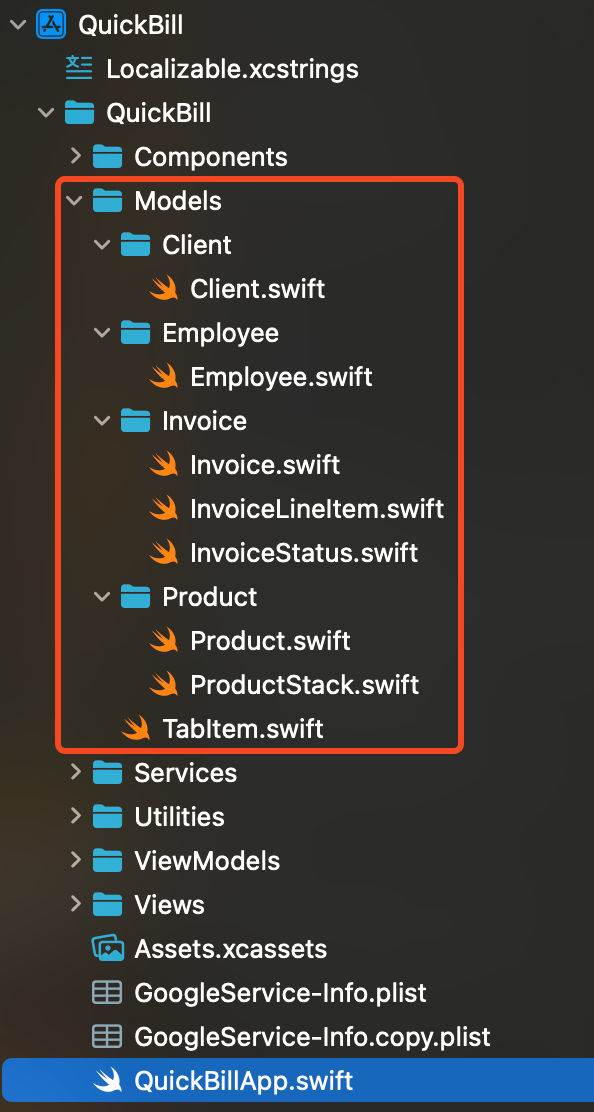
\includegraphics[width=0.5\textwidth]{Ilustraciones/ios_models_folder.png}
\caption{Estructura de la carpeta \textit{Models} en Xcode}
\label{fig:models_folder}
\end{figure}

A continuación se describe brevemente el propósito de cada grupo.

\textit{Models} agrupa todas las entidades que reflejan los documentos de Firestore. Cada subcarpeta contiene un único fichero con la estructura correspondiente:
\begin{itemize}
  \item \textbf{Client/Client.swift}: define la estructura \textit{Client} con campos básicos de la empresa o persona a facturar.
  \item \textbf{Employee/Employee.swift}: representa a cada empleado que accede a la app. Incluye su \textit{userId} (Firebase Auth), nombre, email, teléfono y rol.
  \item \textbf{Invoice}:
    \begin{itemize}
      \item \textit{Invoice.swift}: entidad principal con fechas, importes y referencias a cliente y empleado.
      \item \textit{InvoiceLineItem.swift}: describe cada línea de producto/servicio dentro de una factura.
      \item \textit{InvoiceStatus.swift}: \textit{enum} con los estados \textit{paid}, \textit{pending} y \textit{overdue}.
    \end{itemize}
  \item \textbf{Product}:
    \begin{itemize}
      \item \textit{Product.swift}: catálogo de productos con descripción y precio unitario.
      \item \textit{ProductStack.swift}: colección de productos que se añaden a una factura.
    \end{itemize}
  \item \textit{TabItem.swift}: enumeración con los tabs de navegación de la app.
\end{itemize}

\textit{Services} agrupa la lógica que no depende de la UI pero tampoco encaja como modelo puro:
\begin{itemize}
  \item \textit{AuthService.swift}: envoltorio sencillo sobre Firebase Auth con la finalidad de persistir la sesión de los usuarios en la aplicación.
  \item \textit{InvoicePDFBuilder.swift}: genera el PDF de una factura usando UIGraphicsPDFRenderer; recibe una instancia \textit{Invoice} y devuelve la URL local del fichero.
  \item \textit{InvoiceStatusService.swift}: actualiza el estado de una factura (\textit{paid}, \textit{pending}, \textit{overdue}) según \textit{issuedAt}, \textit{dueDate} y el \textit{status} almacenado.
\end{itemize}

\textit{Utilities} contiene código de soporte reutilizable. Actualmente sólo incluye \textit{AppLanguage.swift}, una enumeración para cambiar el idioma de la interfaz mediante la propiedad \textit{@AppStorage('appLanguage')}.

\textit{ViewModels} se divide en subcarpetas por dominio de negocio:
\begin{itemize}
  \item \textbf{Authentication}: gestiona el inicio de sesión, registro y la opción de 'ovidé mi contraseña'.
  \item \textbf{Clients}: gestión de listado, creación, borrado y edición de clientes.
  \item \textbf{Invoice}: \textit{InvoiceListViewModel.swift}, \textit{InvoiceDetailViewModel.swift} y \textit{AddInvoiceViewModel.swift} para listar, mostrar los detalles y crear nuevas faturas.
  \item \textbf{Products}: ViewModel para el catálogo de productos.
  \item \textbf{Settings}: controla las preferencias de la app.
  \item Además, en la raíz de la carpeta está \textit{AuthViewModel.swift}, que mantiene el estado global de autenticación y se inyecta como \textit{EnvironmentObject}.
\end{itemize}

\textit{Views} organiza las pantallas SwiftUI con la misma lógica de dominios:
\begin{itemize}
  \item \textbf{Authentication}: vistas de inicio de sesión y registro.
  \item \textbf{Clients}: lista de clientes y formulario de creación y edición.
  \item \textbf{Home}: vista inicial tras iniciar sesión (dashboard con todas las facturas).
  \item \textbf{Invoice}: formulario de creación y detalles de las facturas.
  \item \textbf{Products}: listado y formulario de productos.
  \item \textbf{Settings}: ajustes de idioma y cuenta.
  \item \textit{MainTabView.swift}: barra de pestañas inferior que enlaza \textit{Home}, \textit{Products}, \textit{Invoice}, \textit{Clients}, y \textit{Settings}.
  \item \textit{StartView.swift}: pantalla que decide si mostrar la vista de autenticación o el \textit{MainTabView} según el estado de \textit{AuthViewModel}.
\end{itemize}

Esta distribución favorece la separación de responsabilidades, donde los 
ViewModels actúan como enlace entre modelos y vistas, y cada conjunto de vistas se mantiene cohesionado dentro de su propio dominio y los modelos definen la estructura de los datos que se manejan.

\end{large}

\subsection{Generación de PDF}

\begin{large}

En lugar de recurrir a Cloud Functions, la app genera el PDF de la factura localmente a través del servicio \textit{InvoicePDFBuilder}. El proceso se resume a continuación; el código completo puede consultarse en el repositorio público.

\begin{enumerate}
  \item \textbf{Crear el lienzo A4}\newline
  Se instancia un \textit{UIGraphicsPDFRenderer} con tamaño A4 y metadatos del documento:
  \begin{lstlisting}[language=swift, basicstyle=\ttfamily\small, caption={Creación del lienzo A4}]
let bounds = CGRect(x: 0, y: 0, width: 595, height: 842) // A4 @72 dpi
let format = UIGraphicsPDFRendererFormat()
format.documentInfo = [
  kCGPDFContextCreator: "QuickBill",
  kCGPDFContextAuthor : "QuickBill"
]
let renderer = UIGraphicsPDFRenderer(bounds: bounds, format: format)
  \end{lstlisting}

  \item \textbf{Dibujar encabezados}\newline
  Dentro del bloque \textit{renderer.pdfData \{ ctx in …\}}, se escribe el título y los datos de empresa y cliente:
  \begin{lstlisting}[language=swift, basicstyle=\ttfamily\small, caption={Dibujar encabezados}]
ctx.beginPage()
"INVOICE".draw(at: CGPoint(x: bounds.midX-40, y:36),
               withAttributes: titleAttr)

drawBlock(label: "Your company", lines: [businessName])
drawBlock(label: "Bill to", lines: [clientName])
  \end{lstlisting}

  \item \textbf{Renderizar la tabla de productos}\newline
  Se imprime la cabecera y, para cada elemento de \textit{products}, se dibujan descripción, cantidad, precio unitario y total.

  \item \textbf{Calcular importes}\newline
  Al final se muestran subtotal, impuestos, descuentos y el TOTAL resaltado:
  \begin{lstlisting}[language=swift, basicstyle=\ttfamily\small, caption={Calcular importes}]
amountRow("Subtotal",  invoice.subtotal)
amountRow("Tax",       invoice.taxTotal)
amountRow("Discounts", invoice.discounts)
amountRow("TOTAL",     invoice.totalAmount, bold: true)
  \end{lstlisting}

  \item \textbf{Guardar en \textit{Documents}}\newline
  El PDF resultante se escribe como \textit{Invoice-<id>.pdf} en el sandbox de la app y se devuelve la URL para compartir o previsualizar.
\end{enumerate}

Este enfoque permite al usuario generar la factura al instante, sin incurrir en costes adicionales. Para la numeración se reutiliza el \textit{invoice.id} otorgado por Firestore, garantizando unicidad sin contadores globales.

\medskip
\noindent\textit{Código completo:} \url{https://github.com/JuanCarlosAcostaPeraba/QuickBill-App/blob/main/iOS/QuickBill/Services/InvoicePDFBuilder.swift}

\end{large}

\subsection{Autenticación y permisos}

\begin{large}

La autenticación se resuelve con Firebase Auth usando correo y contraseña. La lógica de inicio de sesión se  encapsula en el \textit{SignInViewModel}, mientras que la interfaz se construye en \textit{SignInView}. A grandes rasgos:

\begin{itemize}
  \item \textbf{SignInViewModel.swift}
    \begin{itemize}
      \item Propiedades \textit{@Published} para \textit{email}, \textit{password}, estado de alerta y bandera \textit{didSignIn}.
      \item Método \textit{signIn()} que llama a \textit{Auth.auth().signIn(withEmail:password:)} dentro de una \textit{Task}\,/\textit{await} y gestiona los posibles errores.
    \end{itemize}
  \item \textbf{SignInView.swift}
    \begin{itemize}
      \item Campos \textit{TextField} y \textit{SecureField} enlazados al ViewModel.
      \item Botón “Sign in” que ejecuta \textit{await viewModel.signIn()}; si la autenticación tiene éxito se activa \textit{auth.isSignedIn = true} (estado global mediante \textit{AuthViewModel}).
      \item Enlace a la vista de registro y a la de “Forgot password”.
    \end{itemize}
\end{itemize}

\noindent\textbf{Fragmento clave de autenticación:}
\begin{lstlisting}[language=swift, basicstyle=\ttfamily\small, caption={SignInViewModel.signIn()}]
@MainActor
func signIn() async {
    do {
        _ = try await Auth.auth()
            .signIn(withEmail: email, password: password)
        didSignIn = true
    } catch {
        alertMessage = error.localizedDescription
        showAlert = true
    }
}
\end{lstlisting}

\noindent Una vez autenticado, el UID se usa para filtrar datos, por ejemplo:

\begin{lstlisting}[language=swift, basicstyle=\ttfamily\small, caption={Filtrado de facturas por empleado}]
let uid = Auth.auth().currentUser?.uid ?? ""
Firestore.firestore()
  .collection("businesses")
  .document(businessId)
  .collection("invoices")
  .whereField("employeeId", isEqualTo: uid)
  .getDocuments { snapshot, error in ... }
\end{lstlisting}

El código completo de la pantalla de inicio de sesión, así como del \textit{SignInViewModel}, puede consultarse en GitHub:
\url{https://github.com/JuanCarlosAcostaPeraba/QuickBill-App/tree/main/iOS/QuickBill/Views/Authentication}

\end{large}

\subsection{Filtrado avanzado}

\begin{large}

Para mejorar la usabilidad, se implementó un sistema de filtrado avanzado en la lista de facturas. El usuario puede filtrar por cliente, estado, rango de fechas y rango de importe. Esta funcionalidad se encuentra en \textit{HomeView} y se gestiona a través del \textit{InvoiceListViewModel}.

\begin{lstlisting}[language=swift, basicstyle=\ttfamily\small, caption={HomeView.swift - Filtrado avanzado}]
var filteredInvoices: [Invoice] {
    invoices.filter { inv in
        (selectedStatus == .all || inv.status == selectedStatus) &&
        (
            searchText.isEmpty ||
            inv.companyName.lowercased().contains(searchText.lowercased()) ||
            dateFormatter.string(from: inv.issuedAt).contains(searchText) ||
            String(format: "%.2f", inv.totalAmount).contains(searchText)
        ) && (
            !enableDateFilter ||
            (
                (dateFrom == nil || inv.issuedAt >= dateFrom!) &&
                (dateTo   == nil || inv.issuedAt <= dateTo!)
            )
        ) && (
            !enableAmountFilter ||
            (
                (minTotal == nil || inv.totalAmount >= minTotal!) &&
                (maxTotal == nil || inv.totalAmount <= maxTotal!)
            )
        ) &&
        (selectedClientId == nil || inv.clientId == selectedClientId)
    }
}
\end{lstlisting}

El usuario puede seleccionar el estado de la factura, introducir texto para buscar por cliente o fecha, y activar los filtros de fecha e importe. El resultado se actualiza dinámicamente en la vista.

\end{large}

\subsection{UI/UX y pruebas en simulador}

\begin{large}

La interfaz de usuario se diseñó siguiendo las pautas de Apple para SwiftUI, priorizando la simplicidad y la usabilidad. Se utilizaron componentes estándar como \textit{List}, \textit{Form}, \textit{NavigationView} y \textit{Button} para construir una experiencia coherente.

Se priorizó la accesibilidad y la claridad visual mediante la asignación de colores distintivos a los diferentes estados de las facturas (verde para \textit{paid}, lila para \textit{pending} y rojo para \textit{overdue}), así como la incorporación de animaciones suaves en las transiciones de pantalla. Para la visualización de productos, se optó por \textit{LazyVGrid}, lo que permite una disposición adaptable y eficiente en distintos tamaños de pantalla.

Para verificar que todo funciona, se realizaron pruebas manuales en el simulador de iOS:

\begin{itemize}
  \item Crear una nueva factura: abrir \textit{AddInvoiceView}, rellenar campos, pulsar “Guardar” y comprobar que aparece en \textit{HomeView}.
  \item Editar estado de factura: marcar una factura pendiente como “Paid” y verificar que cambia su color (verde) en la lista.
  \item Generar PDF: pulsar “Generar PDF” en \textit{InvoiceDetailView} y verificar que se guarda en la carpeta \emph{Documents} del simulador.
  \item Inicio de sesión: probar con credenciales correctas e incorrectas para validar la lógica de \textit{Auth}.
\end{itemize}

A continuación se muestran algunas capturas de pantalla que ilustran estos flujos.

\begin{figure}[H]
  \centering
  %------------- Fila 1 -------------
  \begin{minipage}[t]{0.45\textwidth}
    \centering
    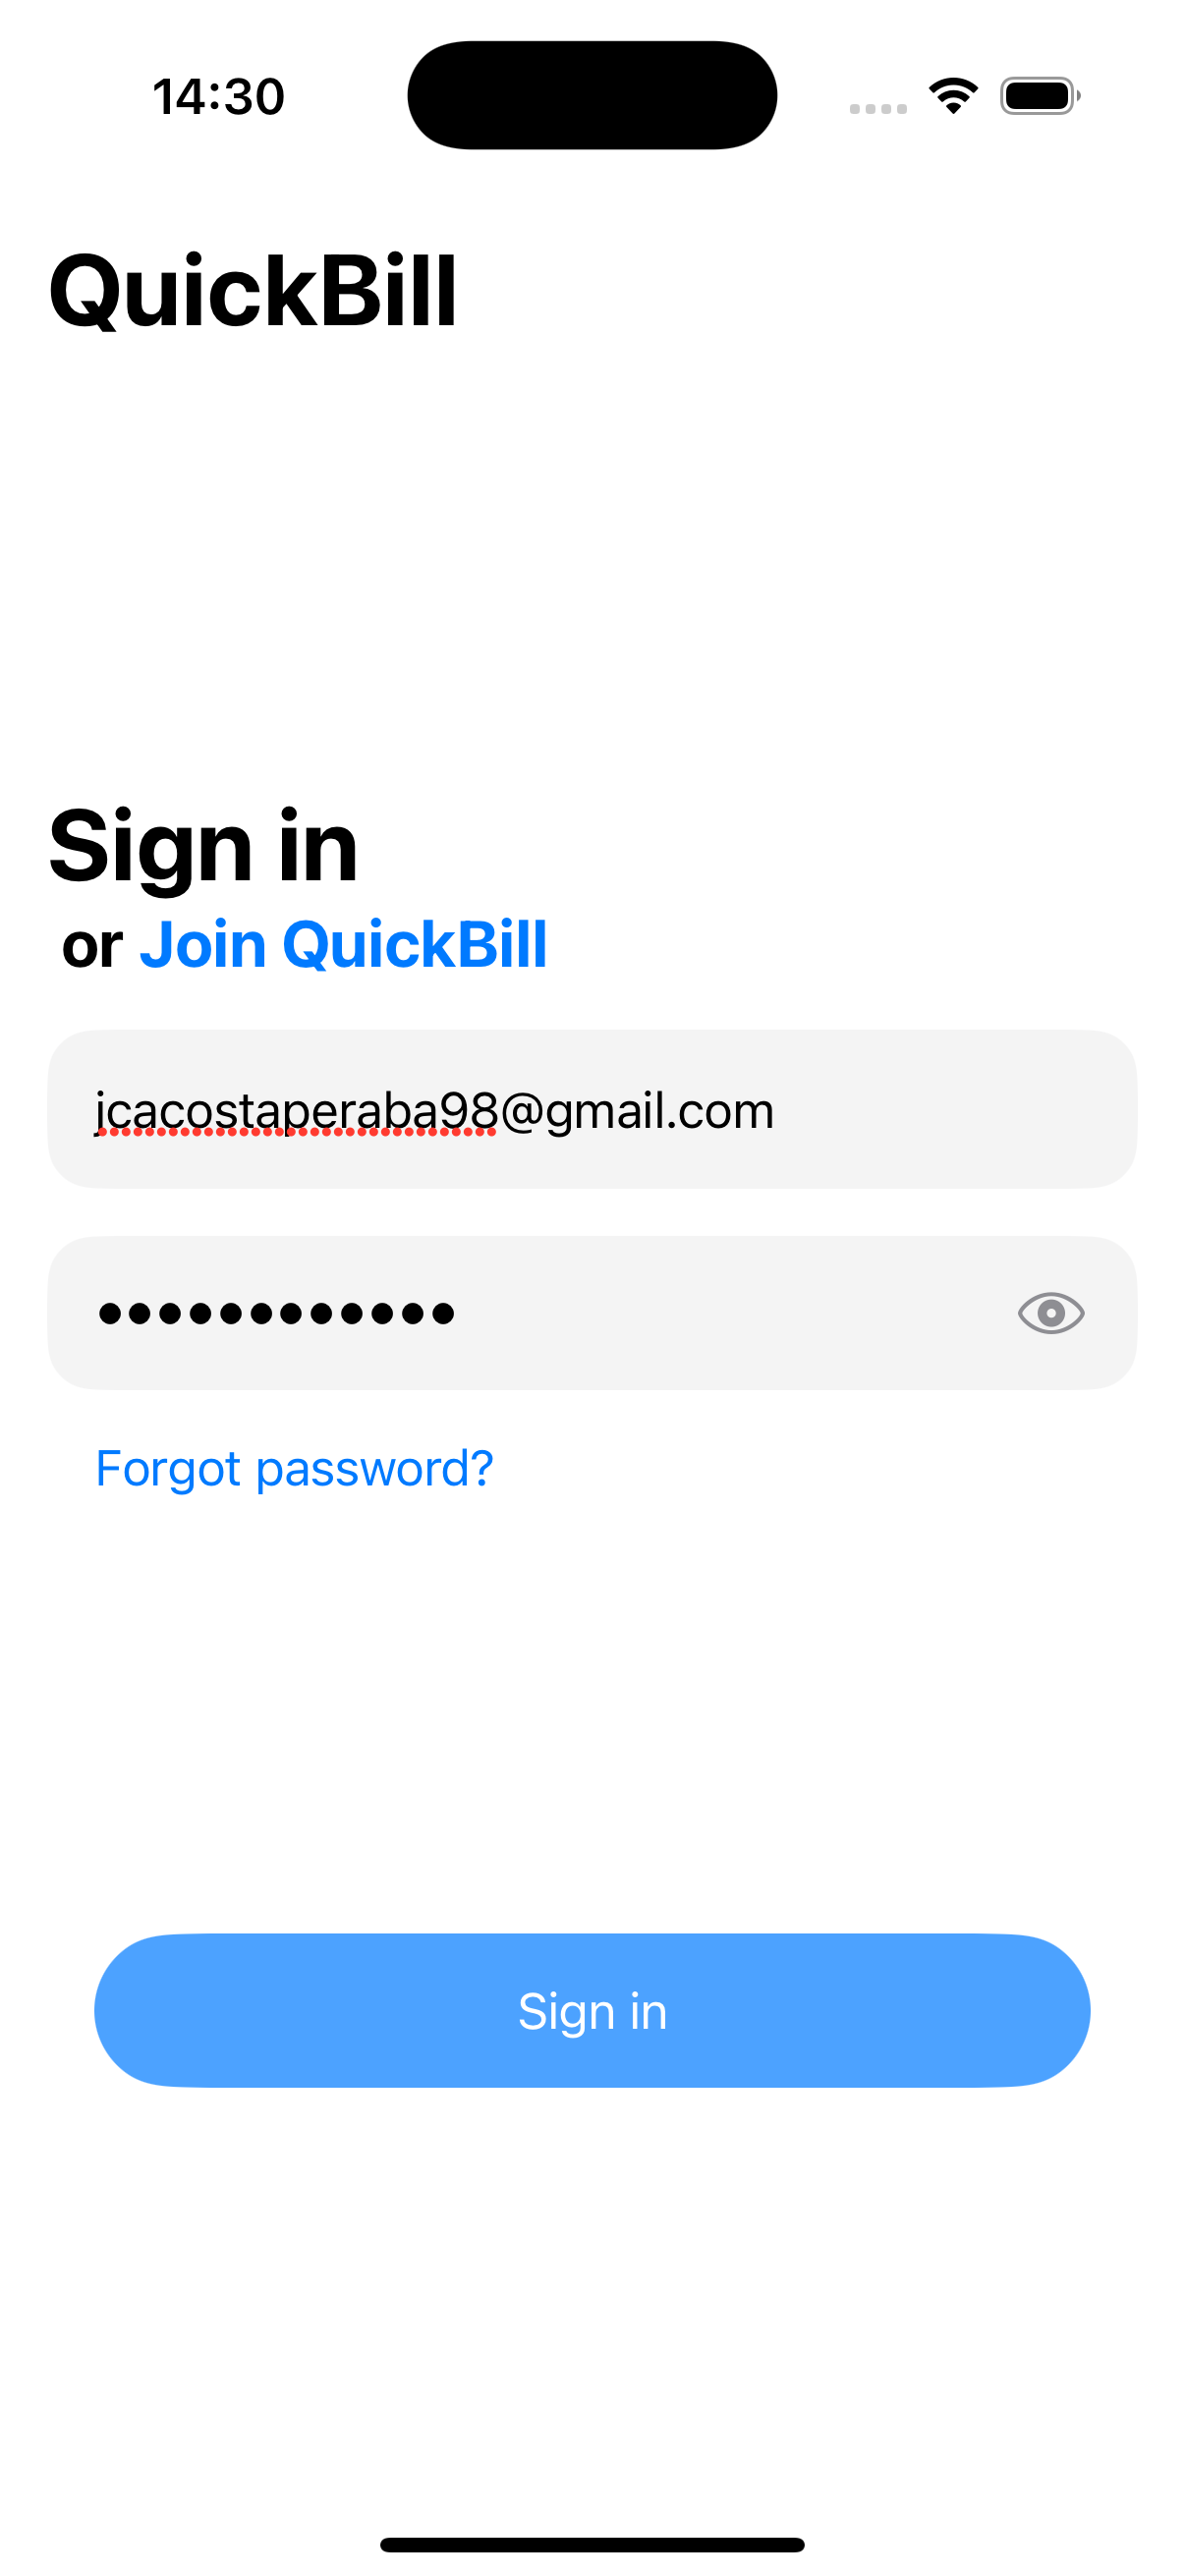
\includegraphics[width=0.8\textwidth]{Ilustraciones/ios_sign_in.png}
    \caption{Pantalla de inicio de sesión}
    \label{fig:ios_sign_in}
  \end{minipage}\hfill
  \begin{minipage}[t]{0.45\textwidth}
    \centering
    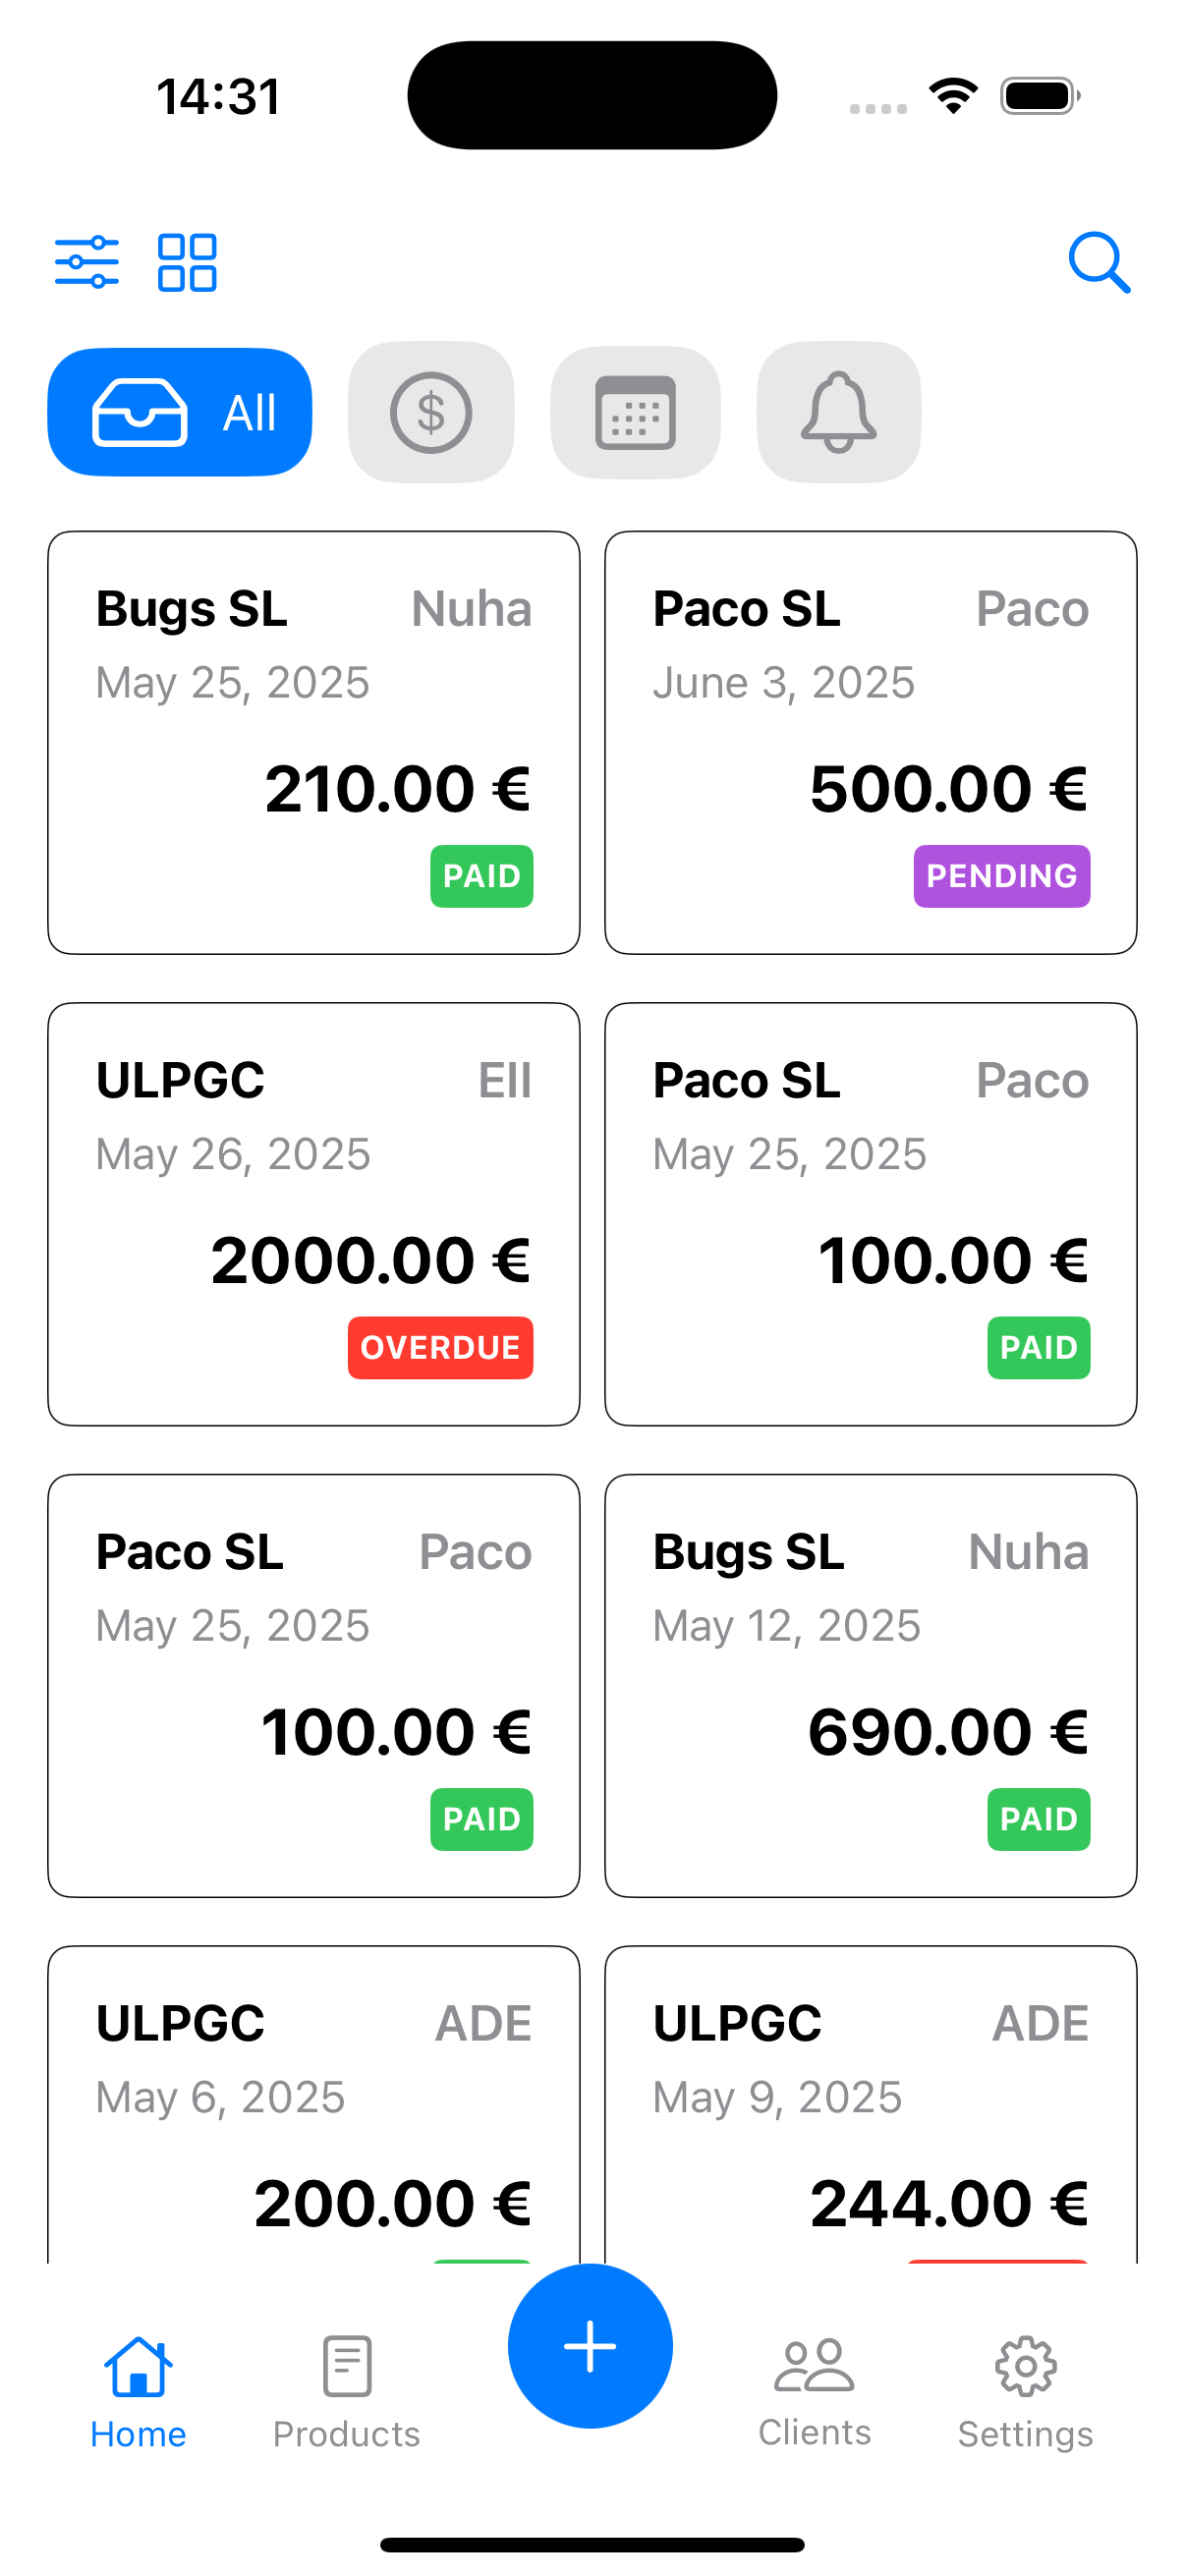
\includegraphics[width=0.8\textwidth]{Ilustraciones/ios_homeview.png}
    \caption{Vista principal con lista de facturas}
    \label{fig:home_view}
  \end{minipage}
\end{figure}

\begin{figure}[H]
	\centering
	%------------- Fila 2 -------------
  \begin{minipage}[t]{0.45\textwidth}
    \centering
    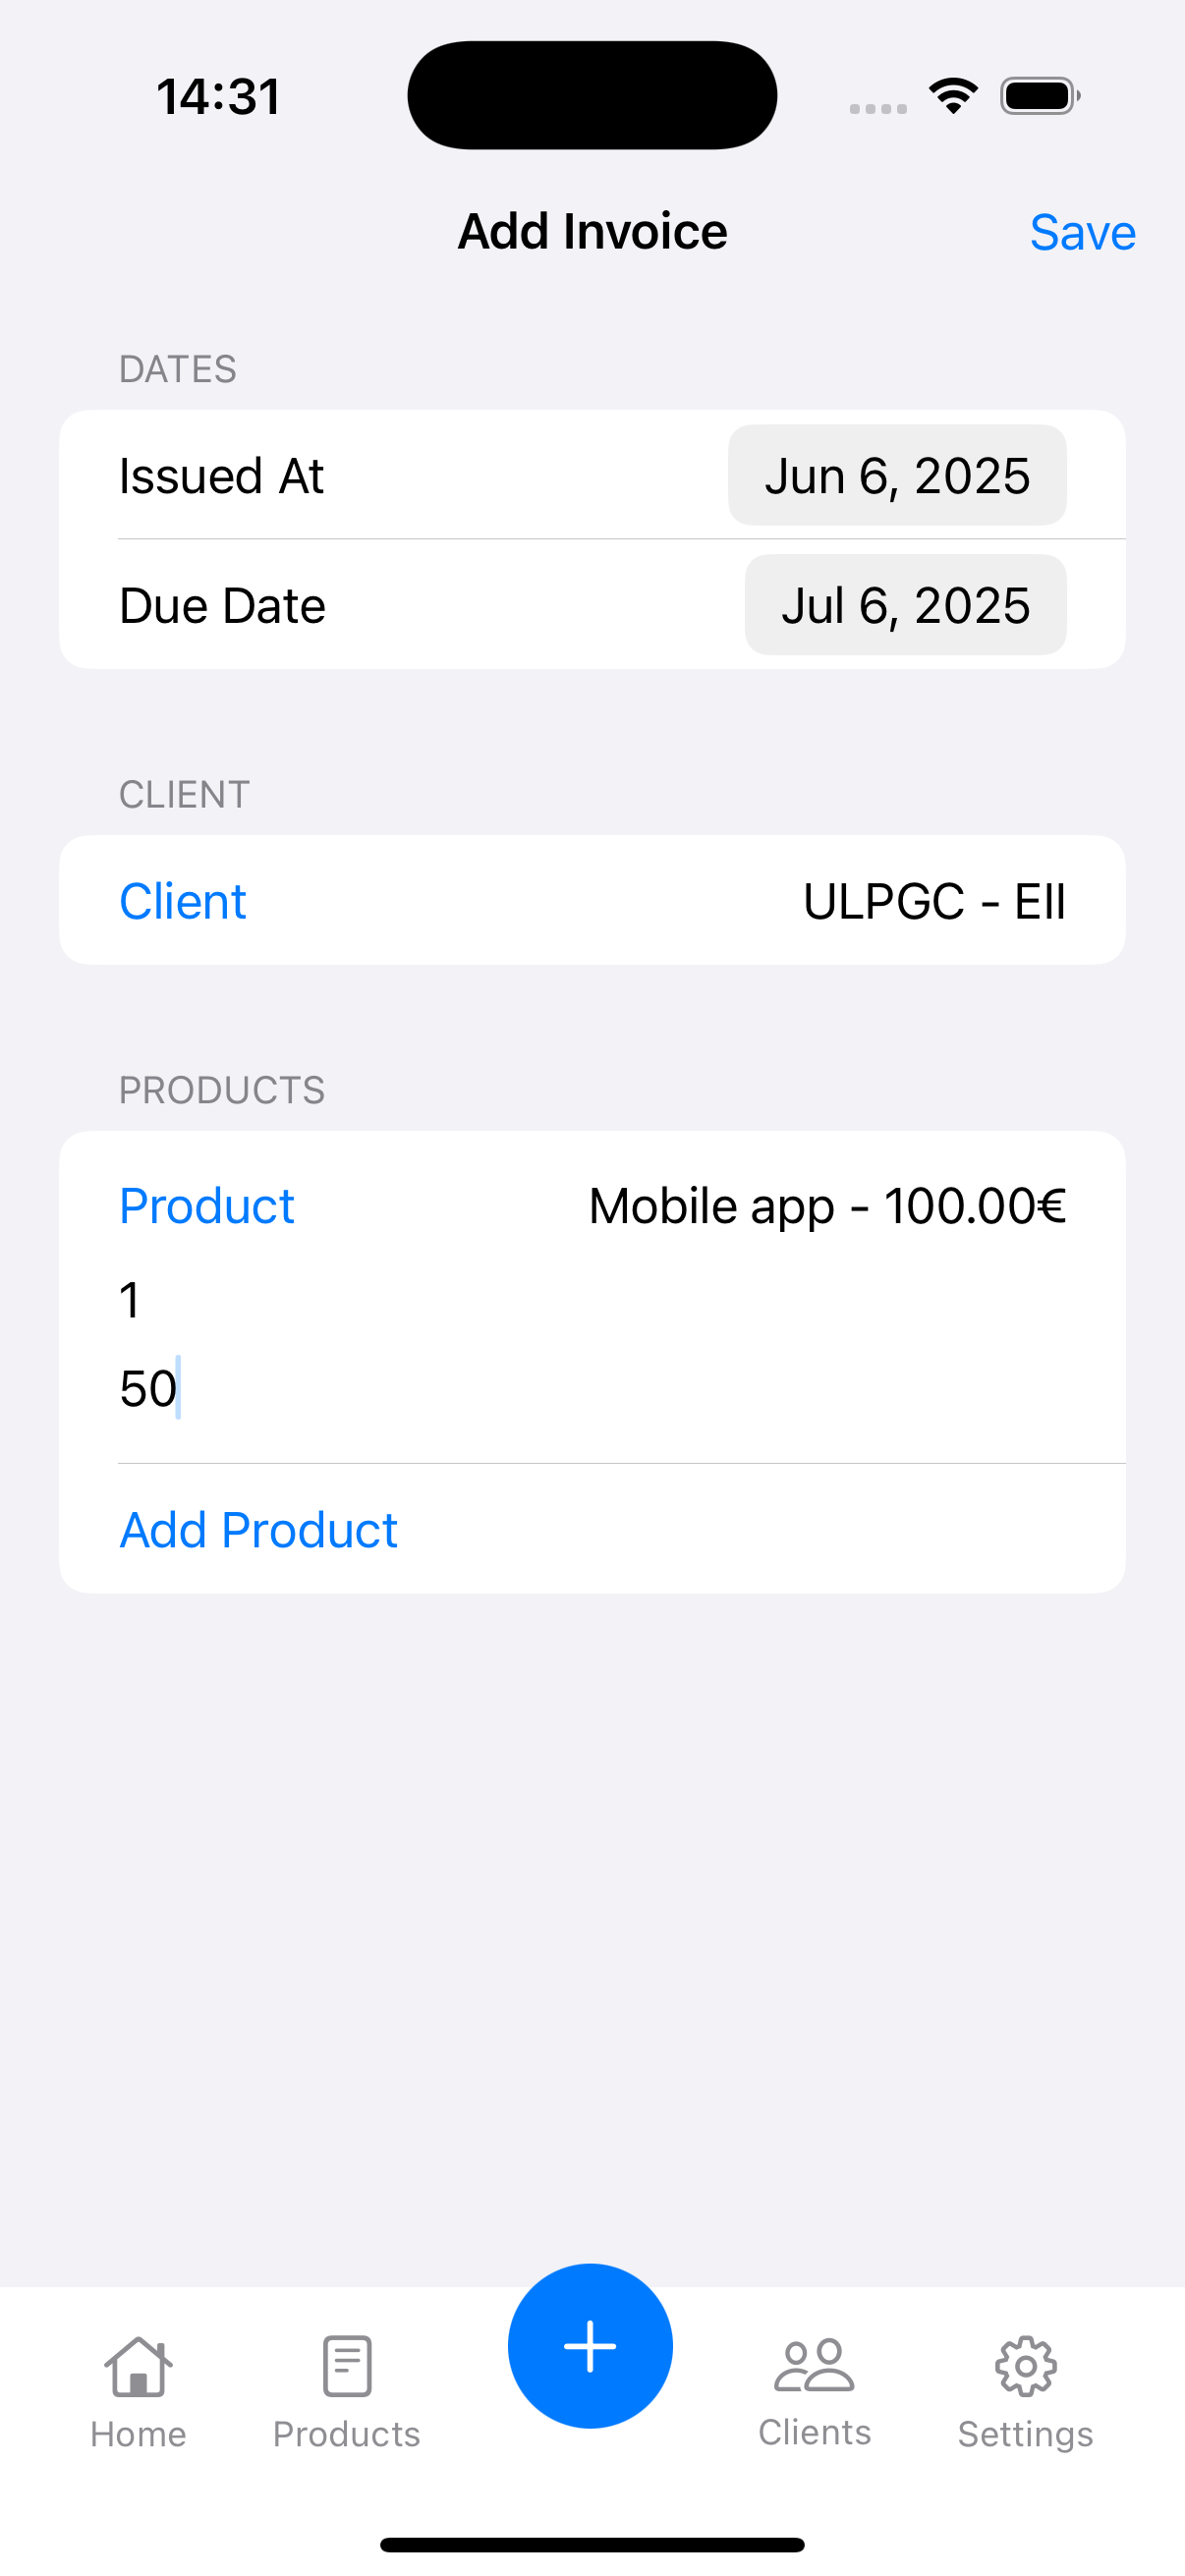
\includegraphics[width=0.8\textwidth]{Ilustraciones/ios_addinvoice.png}
    \caption{Formulario para añadir una nueva factura}
    \label{fig:add_invoice}
  \end{minipage}\hfill
  \begin{minipage}[t]{0.45\textwidth}
    \centering
    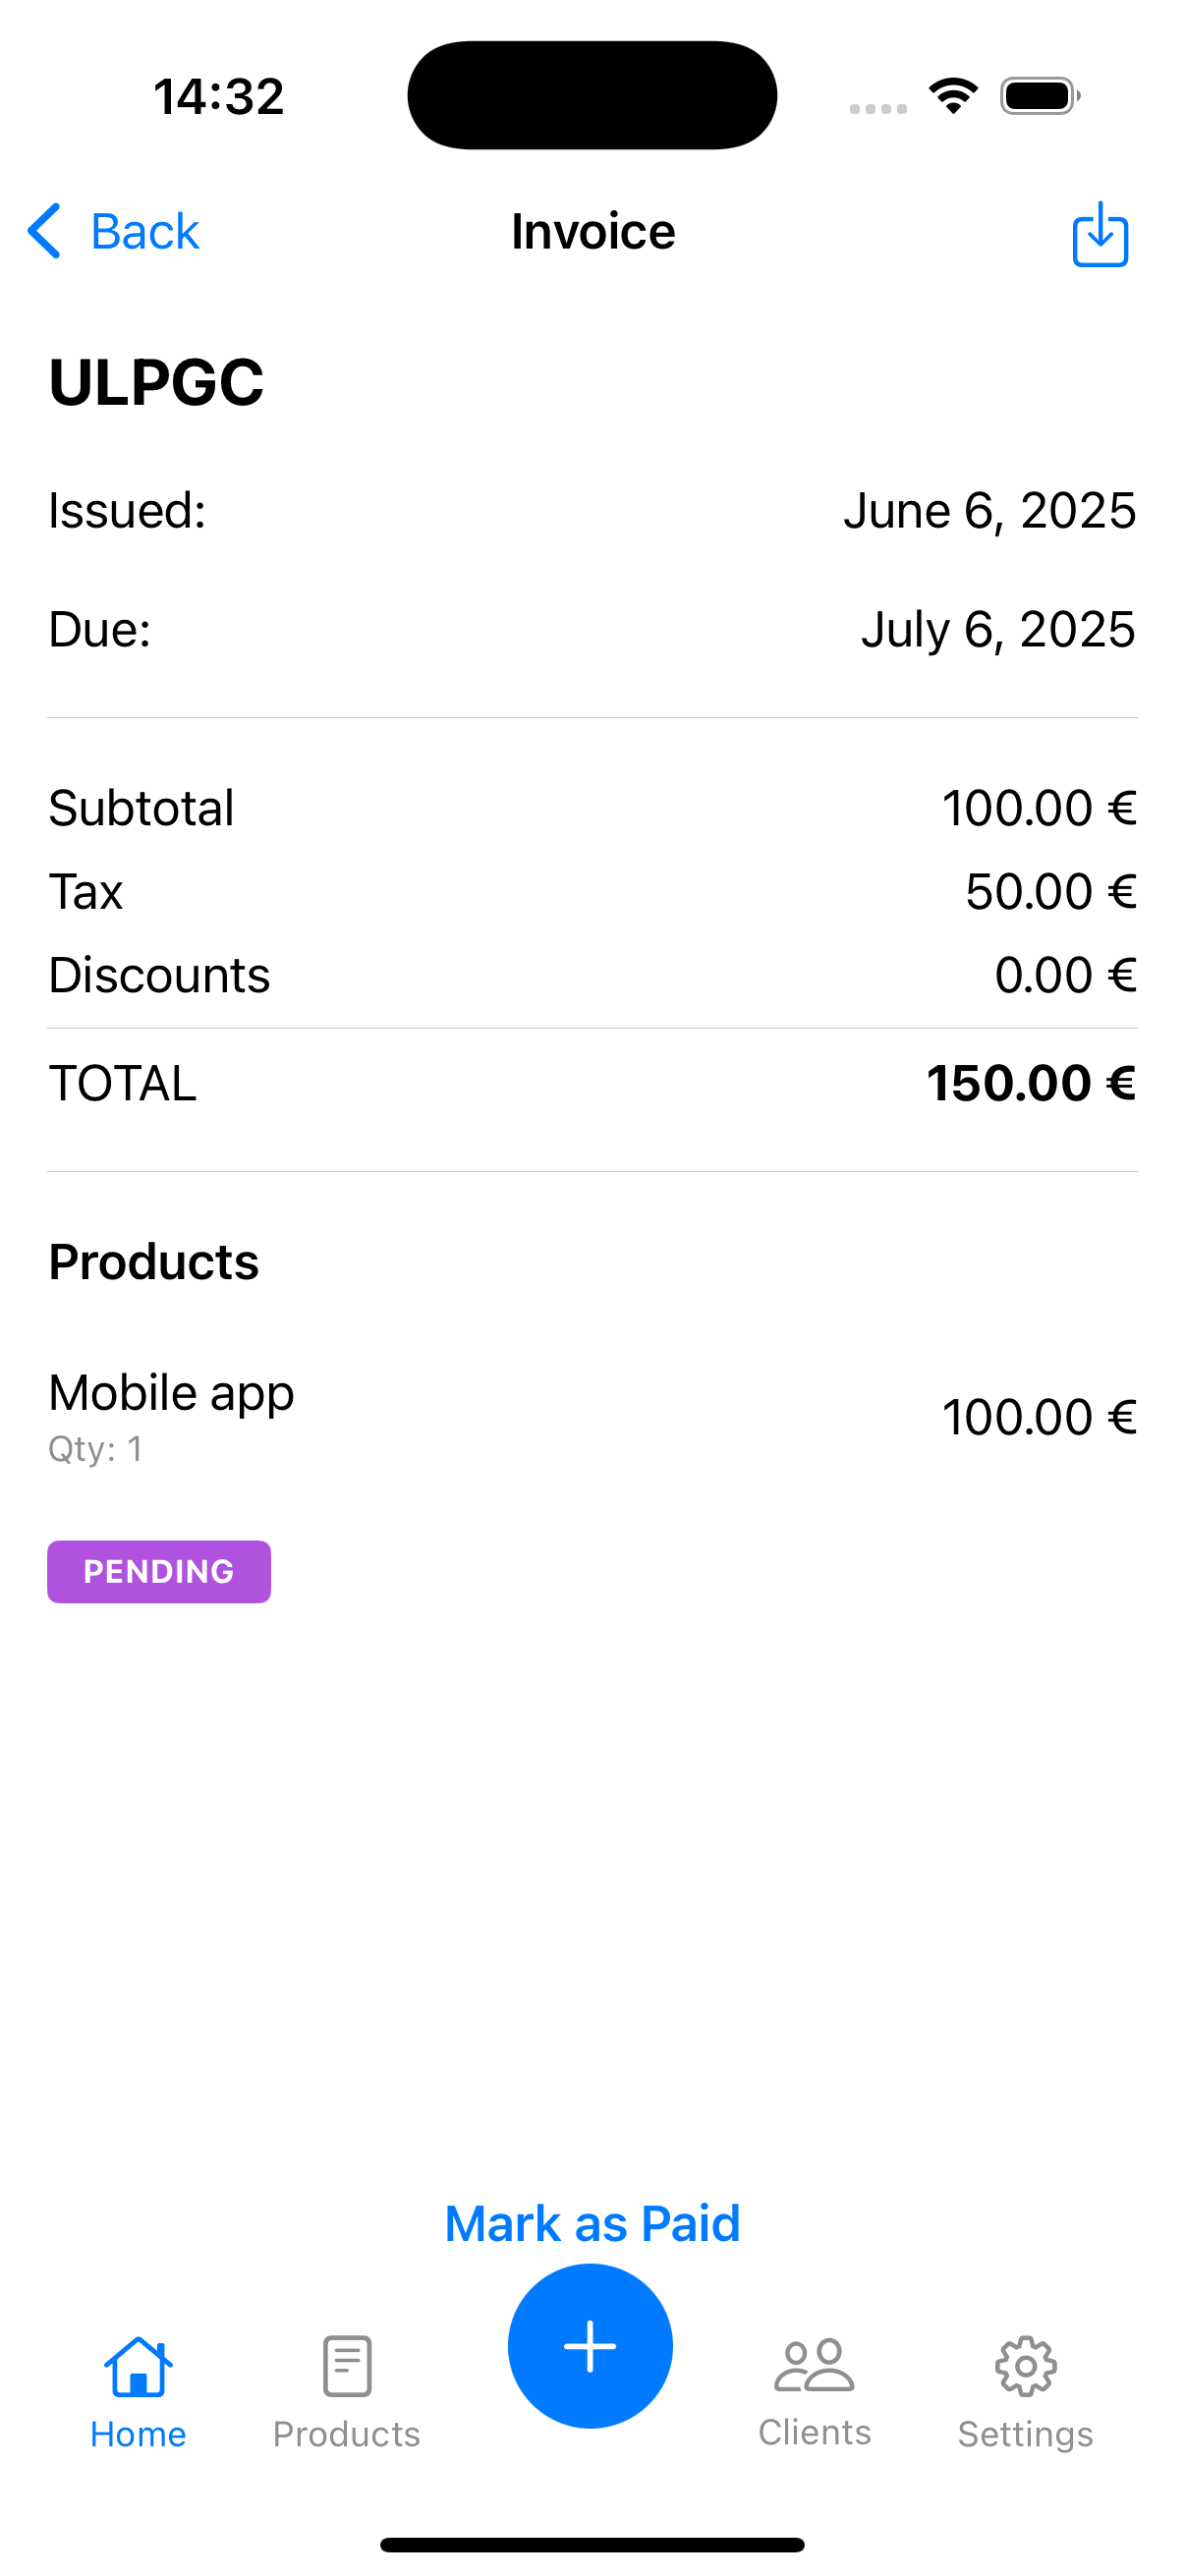
\includegraphics[width=0.8\textwidth]{Ilustraciones/ios_invoicedetails.png}
    \caption{Detalles de una factura con opción de generar PDF}
    \label{fig:invoice_details}
  \end{minipage}
\end{figure}

\begin{figure}[H]
	\centering
	%------------- Fila 3 -------------
  \begin{minipage}[t]{0.45\textwidth}
    \centering
    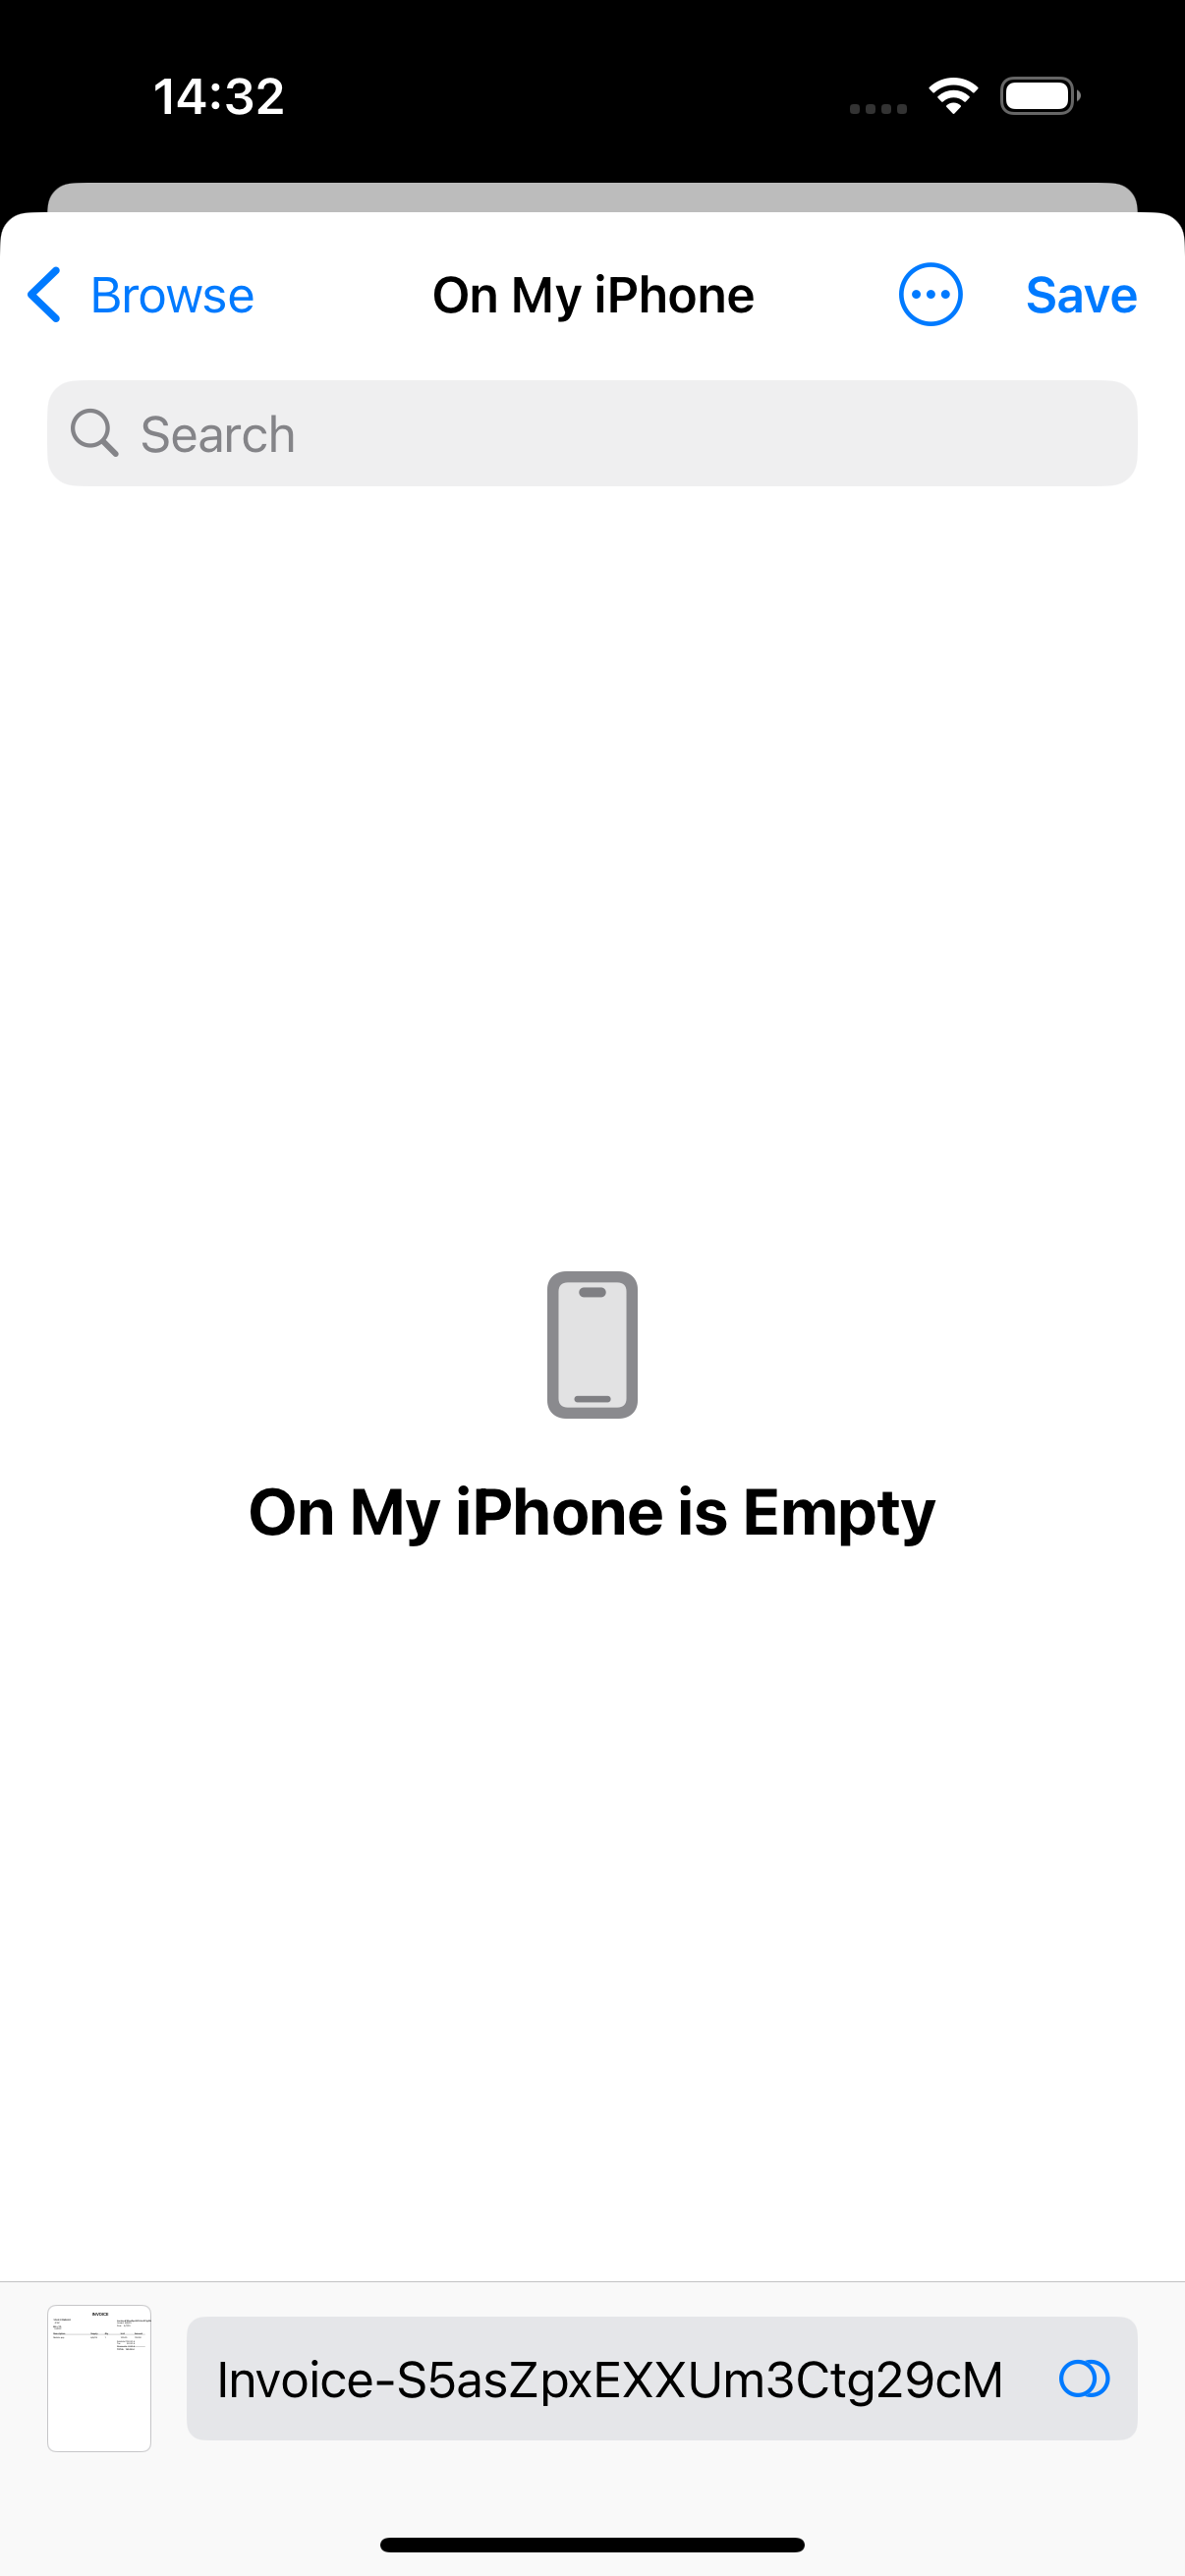
\includegraphics[width=0.8\textwidth]{Ilustraciones/ios_save_pdf.png}
    \caption{Generación del PDF de la factura}
    \label{fig:save_pdf}
  \end{minipage}
\end{figure}

\end{large}

%----------------------------------------------------------
\section{Implementación web}
%----------------------------------------------------------

\begin{large}

La parte web, aunque más ligera, ofrece tres funcionalidades clave: gráfica de pagos mensuales, listado de morosos y tabla con todas las facturas. A continuación se describe su estructura y lógica:

\end{large}

\subsection{Estructura general del proyecto}

\begin{large}

El repositorio para el portal web sigue la convención estándar de Astro:

\begin{figure}[H]
\centering
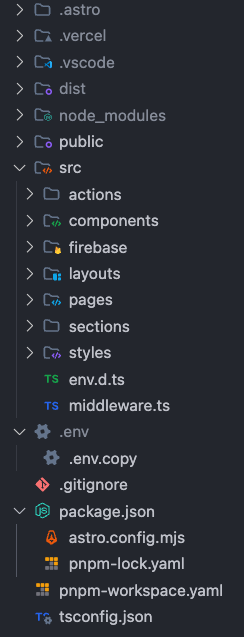
\includegraphics[width=0.3\textwidth]{Ilustraciones/astro_project_structure.png}
\caption{Estructura del proyecto Astro}
\label{fig:astro_project_structure}
\end{figure}

\begin{itemize}
  \item \textit{/src/pages}:
    \begin{itemize}
      \item \textit{index.astro}: página principal que importa los tres componentes.
      \item \textit{login.astro}: página de inicio de sesión para acceder al portal.
    \end{itemize}
  \item \textit{/src/components}:
    \begin{itemize}
      \item \textit{MoneyChart.astro}: renderiza la gráfica de barras usando \emph{lightweight-charts}.
      \item \textit{OverdueList.astro}: muestra tarjetas con clientes morosos y sus importes totales.
      \item \textit{InvoiceTable.astro}: tabla con todas las facturas (cliente, fecha, importe, estado) con ZingGrid.
			\item \textit{Header.astro}: barra de navegación con enlaces a las diferentes secciones y un botón de cierre de sesión.
			\item \textit{ButtonToScrollTop.astro}: botón que permite volver al inicio de la página.
    \end{itemize}
  \item \textit{/src/firebase}:
    \begin{itemize}
      \item \textit{firebase.ts}: inicializa Firebase con la configuración y exporta funciones e instancias de \textit{firestore} y \textit{auth}.
      \item \textit{config.ts}: carga la configuración desde el archivo \textit{.env} y exporta las variables necesarias.
    \end{itemize}
\end{itemize}

\end{large}

\subsection{Carga de datos y renderizado}

\begin{large}

Para cargar los datos de Firestore, se implementaron funciones asíncronas que se invocan en cada componente. A continuación se muestra cómo se obtienen todos los datos relevantes de un usuario a partir de su ID, que es el punto de partida para poblar las tablas y gráficas.

\begin{lstlisting}[language={}, caption={Función para obtener todos los datos de un usuario a partir de su ID}]
async function getAllDataForUser(userId: string) {
	const allData: any = {}

	// 1. get all businesses
	const businessesQuery = await query(collection(firestore, 'businesses'))
	const businessesSnapshot = await getDocs(businessesQuery)
	if (businessesSnapshot.empty) {
		console.log('No businesses found.')
		return []
	}

	// 2. filter all businesses where the user is in the employees collection
	const businesData = businessesSnapshot.docs.map(async (doc) => {
		const businessData = doc.data()
		const businesId = doc.id
		const employees = await getEmployeesBy(businesId)
		const isEmployee =
			employees.filter((employee: any) => employee.userId === userId) || null
		if (!isEmployee || isEmployee.length === 0) {
			return null
		}
		return {
			id: businesId,
			...businessData,
		}
	})
	const businesses = (await Promise.all(businesData)).filter((b) => b !== null)
	if (businesses.length === 0) {
		console.log('No businesses found for this user.')
		return []
	}
	const businessId = businesses[0].id
	allData.businesses = businesses

	// 3. get all invoices that are inside the business collection
	const invoices = getInvoicesBy(businessId)
	allData.invoices = await invoices

	// 4. get all clients that are inside the business collection
	const clients = getClientsBy(businessId)
	allData.clients = await clients

	// 5. get all products that are inside the business collection
	const products = getProductsBy(businessId)
	allData.products = await products

	// 6. get all employees that are inside the business collection
	const employees = getEmployeesBy(businessId)
	allData.employees = await employees

	return allData
}
\end{lstlisting}

Una vez se retorna el objeto \textit{allData}, cada componente puede acceder a los datos necesarios del objeto, el cual se actualizará automáticamente cuando cambien los datos en Firestore.

\begin{lstlisting}[language={}, basicstyle=\ttfamily\small, caption={Función para listar todas las facturas en la tabla}]
function listAllInvoices(allData: any) {
    const invoiceGrid = document.querySelector('#invoiceGrid') as any
    if (!invoiceGrid) return
    const invoiceGridData = allData.invoices.map((invoice: any) => {
        const client = allData.clients.find(
            (client: any) => client.id === invoice.clientId
        )
        return {
            client: client.companyName,
            issued: new Date(invoice.issuedAt.seconds * 1000)
              .toLocaleDateString(
                'es',
                {
                    day: '2-digit',
                    month: '2-digit',
                    year: 'numeric',
                }
            ),
            total: `${invoice.totalAmount}${invoice.currency}`,
            status: invoice.status,
        }
    })
    invoiceGrid.data = invoiceGridData
}
\end{lstlisting}

Para el listado de morosos, \textit{OverdueList.astro} filtra facturas cuyo estado sea “Overdue” y las agrupa por cliente.

\begin{lstlisting}[language={}, basicstyle=\ttfamily\small, caption={Función para listar clientes morosos}]
function listOverdueClients(allData: any) {
	const overdueCards = document.querySelector('#overdueClientsCards')

	let dictOverdueClients: any = {}

	allData.clients.forEach((client: any) => {
		dictOverdueClients[client.id] = {
			name: client.companyName,
			amount: 0,
			currency: '',
		}
	})

	allData.invoices.forEach((invoice: any) => {
		if (invoice.status === 'Overdue') {
			const client = dictOverdueClients[invoice.clientId]
			if (client) {
				client.amount += invoice.totalAmount
				client.currency = invoice.currency
			}
		}
	})
    
	/* Inyectar HTML */
}
\end{lstlisting}

\end{large}

\subsection{Librerías externas}

\begin{large}

Para el portal web se utilizaron varias librerías externas que facilitan la creación de gráficos, tablas y la experiencia de usuario:

\begin{itemize}
\item \textbf{lightweight-charts}: Permite renderizar gráficas de barras y líneas de forma eficiente y responsiva\,\cite{lightweight_charts}. Se emplea en el componente \textit{MoneyChart.astro} para mostrar la evolución mensual de los pagos.
\item \textbf{ZingGrid}: Framework para crear tablas interactivas y personalizables\,\cite{zinggrid}. Se utiliza en \textit{InvoiceTable.astro} para listar todas las facturas con ordenación, filtrado y paginación.
\end{itemize}

Estas librerías permiten construir una interfaz moderna y dinámica, reduciendo el esfuerzo de desarrollo y mejorando la experiencia del usuario final.

\end{large}

\subsection{Despliegue del portal en Vercel}

\begin{large}
	
El portal web se despliega en Vercel siguiendo el flujo de integración continua:

\begin{enumerate}
  \item Cada vez que se hace \emph{push} a la rama \textit{main}, Vercel detecta el cambio y ejecuta el comando \textit{pnpm run build}.
  \item Una vez compilado, Vercel optimiza los activos estáticos y publica el sitio en una URL de producción.
\end{enumerate}

A continuación se muestra una captura del panel de Vercel donde se observa el estado del último despliegue y la URL asignada.

\begin{figure}[H]
\centering
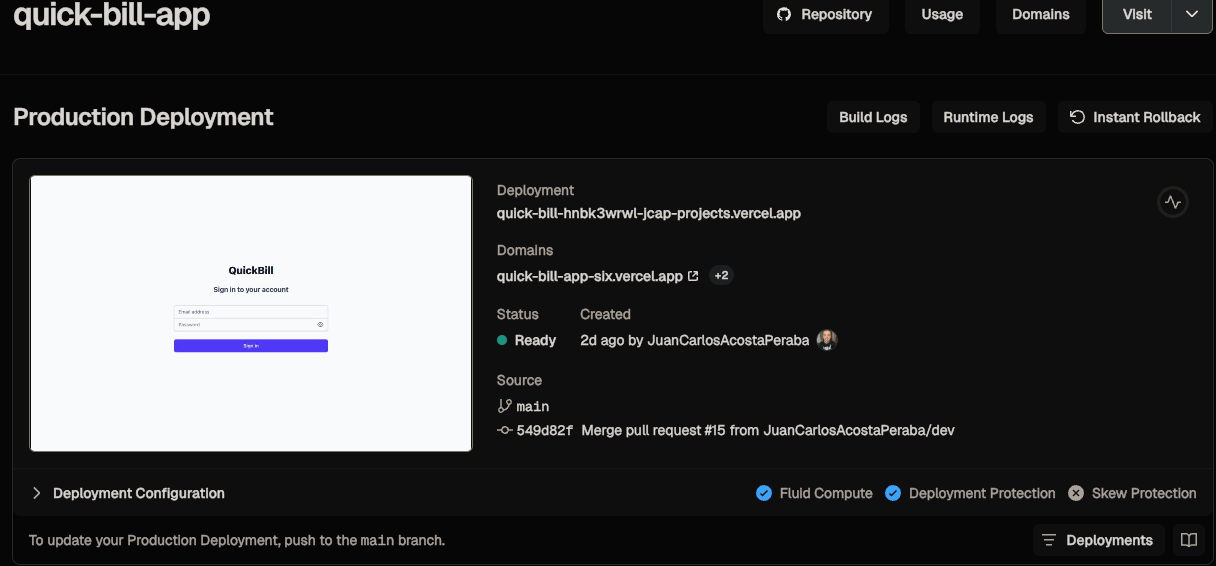
\includegraphics[width=0.8\textwidth]{Ilustraciones/vercel_deploy.png}
\caption{Panel de Vercel con el estado del último despliegue}
\label{fig:vercel_deploy}
\end{figure}

\begin{figure}[H]
\centering
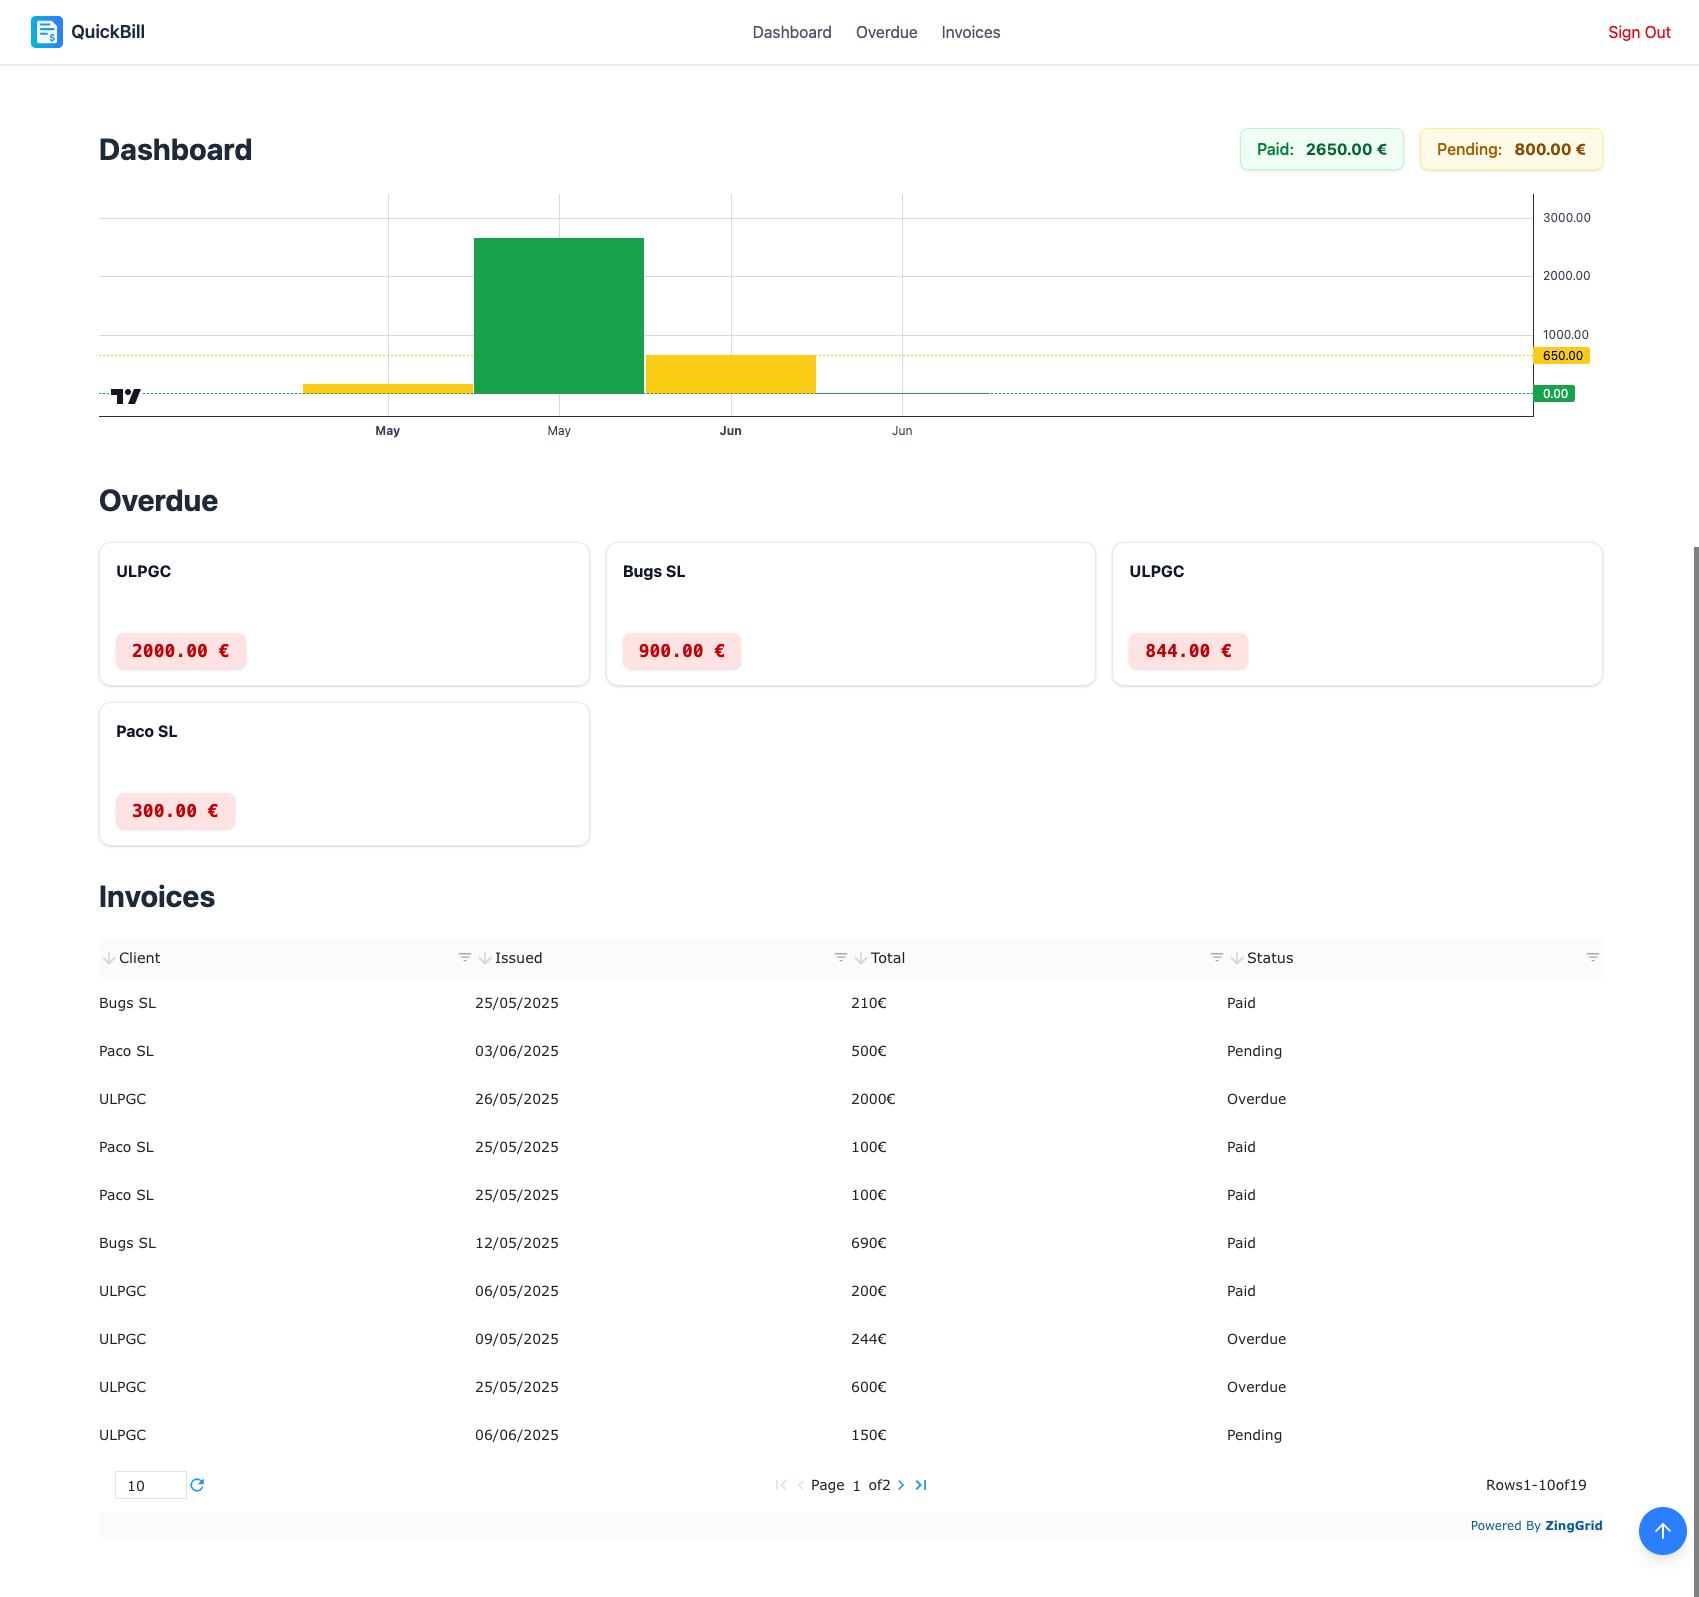
\includegraphics[width=0.8\textwidth]{Ilustraciones/vercel_deployed.png}
\caption{Portal web desplegado en Vercel}
\label{fig:vercel_deployed}
\end{figure}

\noindent El portal web está disponible en la URL \url{https://quick-bill-app-six.vercel.app/}, donde los usuarios pueden iniciar sesión y acceder a las funcionalidades descritas. Algunas cuentas de prueba que se pueden usar son:
\begin{itemize}
	\item \texttt{jcacostaperaba98@gmail.com} / \texttt{qwerty123456}
	\item \texttt{juancarlos@jcap.com} / \texttt{estoEsUnT3st}
\end{itemize}

\end{large}


% 4. Resultados y trabajo futuro
\chapter{Resultados y trabajo futuro}
%----------------------------------------------------------
% Capítulo 4 – Resultados
%----------------------------------------------------------

%----------------------------------------------------------
\section{Resultado}
%----------------------------------------------------------

\begin{large}

La versión actual de la aplicación cumple con los objetivos esenciales planteados en el Capítulo~1:
\begin{itemize}
    \item Gestión completa de facturas: creación, edición, filtrado por estado (\textit{Paid} / \textit{Pending} / \textit{Overdue}) y eliminación.
    \item Catálogo de clientes y productos totalmente operativos.
    \item Generación de PDF directamente en el dispositivo iOS, con numeración única basada en el \texttt{invoice.id} de Firestore.
    \item Portal web accesible con tres vistas clave: gráfica de pagos mensuales, listado de morosos y tabla completa de facturas.
    \item Despliegue continuo en Vercel, con certificados TLS automáticos.
\end{itemize}

\end{large}

\subsection{Desviaciones respecto al plan inicial}

\begin{large}

\begin{itemize}
    \item \textbf{Modo offline}: no llegó a implementarse por limitación de tiempo.
    \item \textbf{App Android}: sólo se completó el esqueleto de proyecto.
    \item \textbf{Cloud Functions y Cloud Storage}: sustituidos por generación y almacenamiento local de PDFs para evitar costes.
\end{itemize}

Aun así, el núcleo funcional se encuentra implementado y operativo, permitiendo emitir facturas y visualizar su estado desde cualquier lugar con conexión.

\end{large}

%----------------------------------------------------------
\section{Conclusión}
%----------------------------------------------------------

\begin{large}

El desarrollo de este proyecto ha puesto de manifiesto el esfuerzo que implica diseñar una plataforma coherente en todas sus capas. Desde la definición del modelo de datos en Firestore hasta la disposición final de cada botón en la pantalla, cada decisión ha requerido un equilibrio entre simplicidad de uso y robustez interna.

\textbf{Arquitectura de la base de datos}

El esquema jerárquico (\texttt{businesses\,/invoices\,/clients\,/employees\,/products}) resultó sencillo de consultar y asegurar, pero elegir una estructura que escalara sin duplicar datos supuso múltiples iteraciones. Hubo que considerar, por ejemplo, qué nivel de anidación permitía aplicar reglas de seguridad sin penalizar el rendimiento; o cómo traducir relaciones \emph{n\,:\,1} (una factura pertenece a un único cliente) a un modelo sin uniones nativas. El resultado es una base de datos que mantiene la coherencia y aísla correctamente la información de cada empresa.

\textbf{Diseño minimalista de la app}

Mostrar solo lo imprescindible en cada pantalla exigió agrupar operaciones y reducir opciones visibles. Se descartaron menús redundantes y se reorganizaron flujos para que el usuario pudiese emitir una factura en menos de un minuto: seleccionar cliente, añadir líneas de producto y pulsar “Guardar”. La navegación basada en pestañas (
\textit{Home}, \textit{Invoices}, \textit{Clients}, \textit{Products}, \textit{Settings}) demostró ser la forma más intuitiva de acceso rápido, y el uso de colores (verde para \textit{Paid}, lila para \textit{Pending}, rojo para \textit{Overdue}) evita distracciones a la vez que señala el estado crítico de cada pago.

\textbf{Lecciones aprendidas}

\begin{itemize}
  \item Separar la lógica de negocio en ViewModels y servicios facilita testear y añadir nuevas funciones sin efectos colaterales sobre la UI.
  \item Definir las reglas de Firestore antes de implementar llamadas previene fugas de seguridad y reduce tiempo de depuración.
  \item El minimalismo en interfaz no implica menos funcionalidad; implica esconder la complejidad hasta que sea necesaria.
\end{itemize}

En conjunto, la plataforma cumple su objetivo principal: ofrecer una solución de facturación ágil y comprensible. El trabajo invertido en la arquitectura de datos y la experiencia de usuario sienta una base sólida para continuar evolucionando la aplicación.

\end{large}

\break

%----------------------------------------------------------
\section{Trabajos futuros}
%----------------------------------------------------------

\begin{large}

Como líneas de evolución se plantean diversas mejoras que consolidarían la plataforma y la harían competitiva frente a soluciones consolidadas:
\begin{enumerate}
  \item \textbf{Modo offline completo}.  Implementar caché local persistente (Core Data + Cloud Kit o SQLite) y un mecanismo de sincronización diferencial con Firestore. De esta forma, el usuario podría emitir facturas sin conexión y la reconciliación de cambios se ejecutaría en segundo plano cuando vuelva la red.
  \item \textbf{OCR y lectura de códigos QR}.  Integrar Vision Kit para capturar facturas de proveedor o tickets y extraer automáticamente importes, fechas e IVA. Además, permitir la lectura de códigos QR europeos (Facturae o Factur-X) para precargar datos de cliente y líneas de producto.
  \item \textbf{Exportación avanzada}.  Añadir exportación a CSV / Excel y conexión directa con herramientas de contabilidad (A3, Contasol, Holded) mediante APIs públicas. Esto facilitará auditorías y conciliaciones bancarias.
  \item \textbf{Firma digital}.  Incluir un flujo opcional para firmar digitalmente la factura, asegurando integridad y no repudio.
  \item \textbf{Automatización de envío}.  Configurar plantillas de correo y adjuntar el PDF firmado directamente desde la app, con opción de recordatorios automáticos a los 7 días y el día de vencimiento.
  \item \textbf{Notificaciones proactivas}.  Enviar notificaciones push o correos cuando una factura vence, cuando el cliente visualiza el PDF o cuando se acerca el umbral de almacenamiento del plan gratuito.
  \item \textbf{Refactorización Android}.  Retomar el esqueleto en Kotlin y completar la paridad funcional con iOS, usando Jetpack Compose y el mismo esquema de Firestore.
  \item \textbf{Dashboard avanzado}.  Añadir nuevos gráficos comparativos y funciones de contabilidad.
\end{enumerate}

Estas mejoras ampliarían el alcance funcional y aportarían valor añadido a autónomos y pymes.

\end{large}


\vspace{1cm}

\bibliography{ref}
\bibliographystyle{unsrtnat}
\clearpage

\printglossary[title={Glosario}]

\end{document}